\documentclass[12pt]{report}
\usepackage[utf8]{vietnam}
\usepackage{graphicx}
%\usepackage{svg}
\usepackage{fancyhdr}
\usepackage{nameref}
\usepackage{parskip}
\usepackage{amssymb}
\usepackage{amsmath}
\usepackage{float}
\usepackage{tikz}
\usepackage{fancybox}
\usetikzlibrary{positioning}
\usepackage[left=3 cm,right=2 cm,top=2cm,bottom=2cm]{geometry}
\usepackage[labelfont=bf]{caption}
\usepackage[hidelinks]{hyperref}
\usepackage[final]{pdfpages}
\usepackage{bookmark}
\usepackage{enumitem}
\usepackage[bottom]{footmisc}
\usepackage{multirow}
\usepackage{array}
\newcolumntype{x}[1]{>{\centering\arraybackslash\hspace{0pt}}p{#1}}

\pagestyle{fancy}
\fancyhf{}
\fancyhead[R]{\normalsize{\textit{\leftmark}}}
\fancyhead[LE,LO]{\thepage}
\renewcommand{\headrulewidth}{0.4pt}

\graphicspath{{images/}}

%-----------------SET PARAMS----------------------------------
\tikzset{
  treenode/.style = {shape=rectangle,
                     draw, align=center,
                     top color=white, bottom color=blue!20},
  root/.style     = {treenode, font=\Large, bottom color=red!30},
  env/.style      = {treenode, font=\ttfamily\normalsize},
  dummy/.style    = {circle,draw}
}

%---------------END OF SET PARAMS---------------------------

\begin{document}

%---------------SET FOR DIAGRAM------------------------------
\usetikzlibrary{arrows,chains,positioning,scopes}

\tikzset{
    block/.style={draw,thick,text width=5em,minimum height=6.5em,minimum width=5em,align=center},
    arrow/.style={->, thick}
}

%------------------TITLE PAGE-----------------------------------
\begin{titlepage}

\newcommand{\HRule}{\rule{\linewidth}{0.5mm}} % Defines a new command for the horizontal lines, change thickness here

\center % Center everything on the page
 
%----------------------------------------------------------------------------------------
%	HEADING SECTIONS
%----------------------------------------------------------------------------------------
\begin{flushright}
\end{flushright}
\textsc{\large ĐẠI HỌC BÁCH KHOA THÀNH PHỐ HỒ CHÍ MINH}\\[0.2cm]
\textsc{\Large \scshape khoa khoa học và kỹ thuật máy tính}\\[0.5cm]
\begin{figure}[H] 
\centering

\includegraphics[scale=1.6]{images/logo.jpg}
\end{figure} 

\textsc{\large BÁO CÁO KỸ THUẬT \\ MÔN KỸ NĂNG CHUYÊN NGHIỆP CHO KỸ SƯ (CO2001)}\\[0.2cm] % Minor heading such as course title

%----------------------------------------------------------------------------------------
%	TITLE SECTION
%----------------------------------------------------------------------------------------
\HRule \\[0.4cm]
{ \huge \bfseries \textcolor{blue}{Xây dựng hệ thống quản lý thư viện \\ sử dụng mã vạch}}\\[0.4cm] % Title of your document
\HRule \\[0.8cm]

%----------------------------------------------------------------------------------------
%	AUTHOR SECTION
%----------------------------------------------------------------------------------------
\begin{flushright}
\begin{minipage}{0.7\textwidth}

\end{minipage}
\end{flushright}

\begin{flushleft} \large
\textbf{Giáo viên hướng dẫn:}\\
GS. TS. Phan Thị Tươi\\
\end{flushleft}

\begin{flushleft} \large
\textbf{Sinh viên thực hiện:}\\
\begin{tabular}{ll}
Nguyễn Văn Đức & \hspace{0.5cm} 1510807\\
Văn Minh Hào & \hspace{0.5cm} 1510901 \\
Hoàng Lê Chánh Tú & \hspace{0.5cm} 1513919\\
Nguyễn Văn Thành & \hspace{0.5cm} 1513056\\[1.5cm]
\end{tabular}
\end{flushleft}

\begin{flushleft} \large
\centering
TP. Hồ Chí Minh, tháng 5 năm 2017
\end{flushleft}

\vfill % Fill the rest of the page with whitespace

\end{titlepage}
%----------------END TITLE PAGE--------------------
\pagenumbering{gobble}
\newpage
	\chapter*{Lời cam đoan}
		\par Chúng tôi xin cam đoan rằng, tất cả mọi kết quả được thể hiện trong bài \textbf{Báo cáo}, ngoại trừ những kết quả được trích dẫn nguồn rõ ràng, đều do chính chúng tôi thực hiện.

		\begin{flushright}
			TP. Hồ Chí Minh, ngày 3 tháng 5 năm 2017
		\end{flushright}

\newpage
	\chapter*{Lời cảm ơn}
		\par Trước tiên, chúng tôi xin gửi lời cảm ơn sâu sắc tới \textbf{GS.TS Phan Thị Tươi}, người đã luôn theo sát và truyền cho chúng tôi những kiến thức rất hữu ích mà cô đã đúc rút được. Những kiến thức này không chỉ giúp chúng tôi thành công trong công việc mà còn trong cả cuộc sống hàng ngày, đối nhân xử thế. Những kiến thức này là hành trang để sau này chúng tôi bước vào đời, trở thành những kỹ sư giỏi chuyên môn, sáng tâm hồn, xứng đáng với hai chữ \textbf{Bách Khoa} mà không phải may mắn chúng tôi mới được học ở ngôi trường này. Môn học \textbf{Kỹ năng chuyên nghiệp cho kỹ sư} quả thật là những gì mà những kỹ sư tương lai như chúng tôi cần và may mắn thay, dưới ngôi trường Đại học Bách Khoa TP.HCM, chúng tôi đã được học môn này và may mắn hơn nữa là được chính GS.TS Phan Thị Tươi trực tiếp truyền lại những kinh nghiệm, kiến thức mà cô đã đúc rút trong quá trình nghiên cứu, giảng dạy và làm việc của mình. Một lần nữa, xin cảm ơn cô. \\Cuối cùng, xin cảm ơn những con người tuyệt vời ở ngôi trường Đại học Bách Khoa TP.HCM đã đồng hành cùng chúng tôi trong suốt thời gian thực hiện Đề tài này.
\newpage
	\chapter*{Lời mở đầu}	
	\label{chpt:abstraction}	
		\par Ở bất kỳ thời kỳ lịch sử này, Thư viện luôn đóng một vai trò cực kỳ quan trọng trong sự phát triển của nhà nước hay con người. Thư viện được coi là kho tri thức của loài người, nhu cầu sử dụng thư viện rất rộng rãi và hầu như tất cả các lĩnh vực đều cần đến Thư viện.
		\par Cùng với sự phát triển của con người, Thư viện theo đó cũng phát triển và hình thành những hình thái và quy mô khác nhau. Theo thời gian, kho tàng tri thức của nhân loại ngày càng tăng lên, cũng bởi lý do đó Thư viện càng đa dạng về nội dung và lớn về số lượng. Nhiều Thư viện có tới hàng vạn cuốn sách, báo, tạp chí và số lượng lớn độc giả đến mượn - trả sách mỗi ngày. Điều đó gây khó khăn cho việc quản lý bằng phương pháp truyền thống.
		\par Với sự ra đời và phát triển mạnh mẽ của công nghệ thông tin, việc quản lý Thư viện trở nên dễ dàng hơn bao giờ hết. Kết hợp hiệu năng tính toán mạnh mẽ của máy tính cùng với mã vạch, chúng ta đã làm giảm đi đáng kể sự phức tạp trong việc quản lý. Công nghệ này đã ra đời khá lâu và tỏ ra khá hiệu quả. Vì lẽ đó, chúng tôi quyết định thực hiện dự án này với mục tiêu thiết kế được một ứng dụng quản lý Thư viện kết hợp với mã vạch để thấy rõ được cách con người đã sử dụng nó như thế nào và hiệu quả mà nó mang lại.
		\par Bài \textbf{Báo cáo} được tổ chức thành 5 chương có cấu trúc như sau:\\
		\textbf{Chương 1} nêu ra vấn đề và giới thiệu đề tài \textbf{\textit{Xây dựng hệ thống quản lý thư viện sử dụng mã vạch}}, chương này cũng đồng thời nói về phạm vi và mục đích của đề tài. Ngoài ra, chương này cũng đưa ra những yêu cầu đối với sản phẩm mà Đề tài hướng đến.\\
		\textbf{Chương 2}, chúng tôi sẽ nói về một số định nghĩa và các công cụ được sử dụng trong Đề tài lần này. \\
		\textbf{Chương 3} nói về việc phân tích và thiết kế hệ thống. \\
		\textbf{Chương 4} mô tả về ứng dụng sa khi hoàn thành\\
		Cuối cùng, \textbf{Chương 5} là phần tổng kết lại đề tài, những điểm hạn chế và hướng phát triển.
		\par Vì kiến thức còn hạn chế, ứng dụng của chúng tôi sẽ có một số thiếu sót so với những ứng dụng đã được tung ra thị trường hay được sử dụng trong các hệ thống Thư viện. Vì vậy, rất mong nhận được sự góp ý từ các bạn. 
		\begin{flushright}
			Nhóm tác giả.
		\end{flushright}

\newpage
	\thispagestyle{empty}
	\pdfbookmark{\contentsname}{Mục lục}
	\tableofcontents	

	\newpage
	\pagenumbering{arabic}
  	\addcontentsline{toc}{chapter}{Danh sách hình vẽ}
	\listoffigures

\newpage		
	\chapter{Giới thiệu đề tài}	
		\label{introduction_chapter}
		\section{Giới thiệu về đề tài}
		\par Trong những năm gần đây, việc tin học hóa các vấn đề trong đời sống ngày càng được phát triển mạnh. Cũng bởi lý do đó, việc ứng dụng CNTT vào việc quản lý Thư viện cũng là một lẽ đương nhiên.
		\par Nhu cầu học tập, nghiên cứu, giải trí của con người ngày càng cao và việc đảm bảo các kiến thức, thông tin là chính xác, logic. Vì vậy, các hệ thống Thư viện lớn ngày nay đã tăng số sách về cả số lượng lẫn thể loại.
		\par Vì thế mà người thủ thư (\textbf{\textit{Librarian}}) trong một ngày phải liên tục lặp đi lặp lại công việc tìm sách, cho độc giả mượn-trả sách, sắp xếp sách đúng theo vị trí quy định đã khó khăn lại càng khó khăn hơn.
		\par Từ đó vấn đề quản lý sách được coi là rất cần thiết. Quản lý tốt cung cấp đầy đủ, nhanh chóng và chính xác về các loại sách cho độc giả và thống kê báo cáo với ban quản lý là thực sự cần thiết.
		\par Quản lý Thư viện là một chuỗi công việc rất vất vã và tốn nhiều công sức. Việc ứng dụng CNTT các hệ quản trị CSDL sẽ giúp cho việc quản lý dễ dàng hơn, tính chính xác cao hơn và hơn nữa, khả năng truy xuất thông tin nhanh hơn. Ngoài ra, việc kết hợp mã vạch đã được ứng dụng từ lâu và tỏ ra rất hiệu quả nên và như đã giới thiệu trong phần \textbf{\nameref{chpt:abstraction}}, đó cũng là lý do mà nhóm chúng tôi chọn thực hiện đề tài này.
		\section{Mục tiêu và phạm vi của Đề tài}
			\subsection{Mục tiêu}
			\begin{itemize}
				\item{Phân tích, thiết kế hệ thống quản lý Thư viện, giảm bớt gánh nặng cho thủ thư.}
				\item{Triển khai ứng dụng bằng một phần mềm cụ thể với giao diện dễ sử dụng.}
			\end{itemize}
			\subsection{Phạm vi đề tài}
			\begin{itemize}
				\item{Đề tài được thực hiện trong phạm vi những kiến thức đã học về hệ quản trị CSDL.}
				\item{Vì là phần mềm Quản lý Thư viện nên ứng dụng quan tâm chủ yếu đến yêu cầu thực tế là công việc của người thủ thư như quản lý sách, quản lý độc giả, quản lý mượn-trả sách,...}
				\item{Phạm vi của Đề tài hướng tới những Thư viện với quy mô lớn(có khoảng từ 10.000 đầu sách), lúc này sẽ thấy rõ được tác dụng, sức mạnh của Đề tài.}
			\end{itemize}		
		\section{Yêu cầu hệ thống}
			\begin{itemize}
				\item{Giao diện đẹp, thân thiện, dễ sử dụng.}
				\item{Tốc độ truy xuất nhanh.}
				\item{Có khả năng sao lưu và khôi phục dữ liệu khi có sự cố xảy ra.}
				\item{Khi thay đổi-thêm một chức năng không làm ảnh hưởng đến các chức năng khác.}
				\item{Có các chức năng cơ bản của một ứng dụng quản lý Thư viện: }
					\begin{itemize}
						\item Tra cứu, thêm, cập nhật sách.
						\item Tra cứu, thêm, cập nhật độc giả.
						\item Quản lý mượn, trả sách.
						\item Thống kê hàng tháng.
					\end{itemize}
			\end{itemize}	
	\chapter{Một số định nghĩa và các công cụ sử dụng}
		\label{definition_chapter}				
		\section{Một số định nghĩa}
		\par Dưới đây chúng tôi sẽ nhắc lại một số định nghĩa về cơ sở dữ liệu liên quan đến đề tài:
			\begin{itemize}
			\item{\textbf{Cơ sở dữ liệu (Database):}} là tập hợp các dữ liệu có cấu trúc và liên quan với nhau được lưu trữ trên máy tính, được nhiều người sử dụng và được tổ chức theo một mô hình.\footnote{\url{https://voer.edu.vn/c/co-so-du-lieu/d11e79e2}}
			\item{\textbf{Hệ quản trị cơ sở dữ liệu (Database Management System):}} là tập hợp các phần mềm cho phép định nghĩa các cấu trúc để lưu trữ thông tin trên máy, nhập dữ liệu, thao tác trên các dữ liệu đảm bảo sự an toàn và bí mật của dữ liệu.\footnote{\url{https://voer.edu.vn/c/co-so-du-lieu/d11e79e2}}
			\item{\textbf{Thực thể (Entity):}} là đối tượng mà ta cần quan tâm trong công tác quản lý. \footnote{\url{https://voer.edu.vn/c/so-do-thuc-the-lien-ket-erd/21aca16d/299b60d4\#}}\\
			Một đối tượng có thể là:
				\begin{itemize}
					\item{Rất cụ thể: }Nhân viên của một cơ quan hay Hóa đơn một dịch vụ,...
					\item{Hoặc trừu tượng: }Khoa Máy tính, Ngành Khoa học máy tính,...
					\item{Thực thể bao gồm các thuộc tính đặc trưng cho thực thể đó, có nhiều loại thuộc tính khác nhau như:}
					\begin{itemize}
						\item{\textbf{Thuộc tính đơn (Single Attribute):}} là thuộc tính không thể phân chia thành các thành phần nhỏ hơn.
						\item{\textbf{Thuộc tính phức hợp (Composite Attribute):}} là thuộc tính có thể phân chia thành những thuộc tính nhỏ hơn, biểu diễn các thuộc tính cơ bản hơn với các ý nghĩa độc lập.
						\item{\textbf{Thuộc tính đơn trị (Attribute):}} là những thuộc tính có giá trị duy nhất cho một thực thể cụ thể.
						\item{\textbf{Thuộc tính đa trị (Multivalued Attribute):}} là thuộc tính có thể có một tập giá trị cho cùng một thực thể.
						\item{\textbf{Thuộc tính khóa (Key Attribute):}} là thuộc tính dùng để xác định thực thể, phân biệt thực thể này với thực thể khác.
						\item{\textbf{Thuộc tính dẫn xuất (Derived Attribute):}} là thuộc tính của thực thể mà có thể truy xuất được thông qua các thuộc tính khác.
					\end{itemize}					
				\end{itemize}
			\item{\textbf{Mô hình thực thể - liên kết:} gọi tắt là mô hình ER (Entity - Relationship Model). Là một mô hình dữ liệu tập trung vào các cấu trúc dữ liệu và các ràng buộc. Thường được sử dụng để thiết kế các ứng dụng cơ sở dữ liệu và nhiều công cụ thiết kế cơ sở dữ liệu sử dụng khái niệm của nó}
			\end{itemize}
			Một số ký hiêu sử dụng trong mô hình ER được mô tả ở \textbf{Hình \ref{fig:attributes}.}
					\begin{figure}
						\centering
						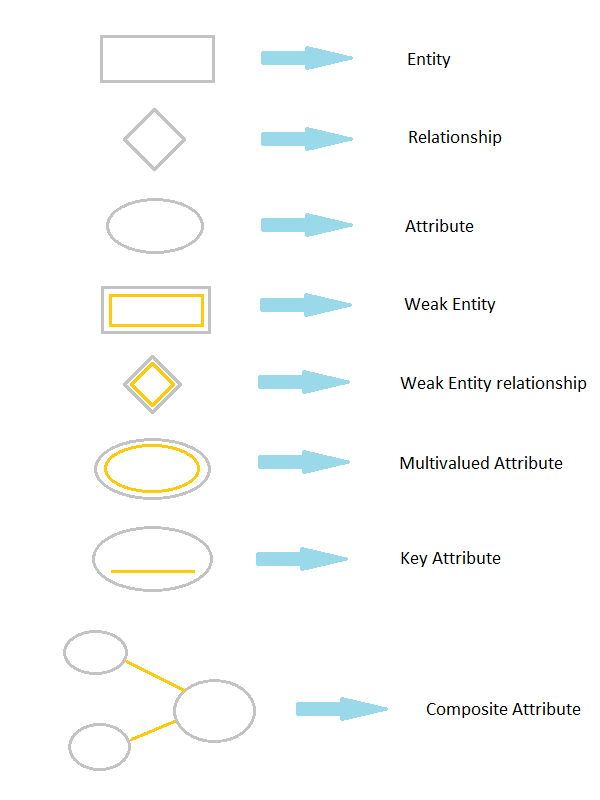
\includegraphics[scale=0.6]{images/ERsymbols.png}
						\caption[Một số ký hiệu trong sơ đồ quan hê ER]{Một số ký hiệu trong sơ đồ quan hê ER \protect\footnotemark{}}
						\label{fig:attributes}
					\end{figure}
					\footnotetext{\url{http://www.studytonight.com/dbms/er-diagram.php}}
		\par Ngoài ra, trong Đề tài này, chúng tôi sử dụng mã vạch (\textbf{\textit{barcode}}) với hai mục đích đó là lưu mã sách và thứ hai là mã của nhân viên hay độc giả. Việc sử dụng mã vạch đơn giản hóa các công việc quản lý cũng như tìm kiếm, mượn - trả sách. Dưới đây là định nghĩa ngắn gọn về mã vạch:
				\begin{itemize}
					\item{\textbf{Mã vạch} là sự thể hiện thông tin trong các dạng nhìn thấy trên các bề mặt của sản phẩm, hàng hóa mà máy móc có thể đọc được. Mã vạch lưu trữ dữ liệu theo bề rộng của các vạch được in song song cũng như của khoảng trống giữa chúng. Nội dung của mã vạch là thông tin về sản phẩm như: Nước đăng ký mã vạch, tên doanh nghiệp, lô, tiêu chuẩn chất lượng đăng ký, thông tin về kích thước sản phẩm, nơi kiểm tra...} \footnote{\url{http://marketingbox.vn/Ma-vach-la-gi.html}}
					\begin{figure}[H]
					\centering
					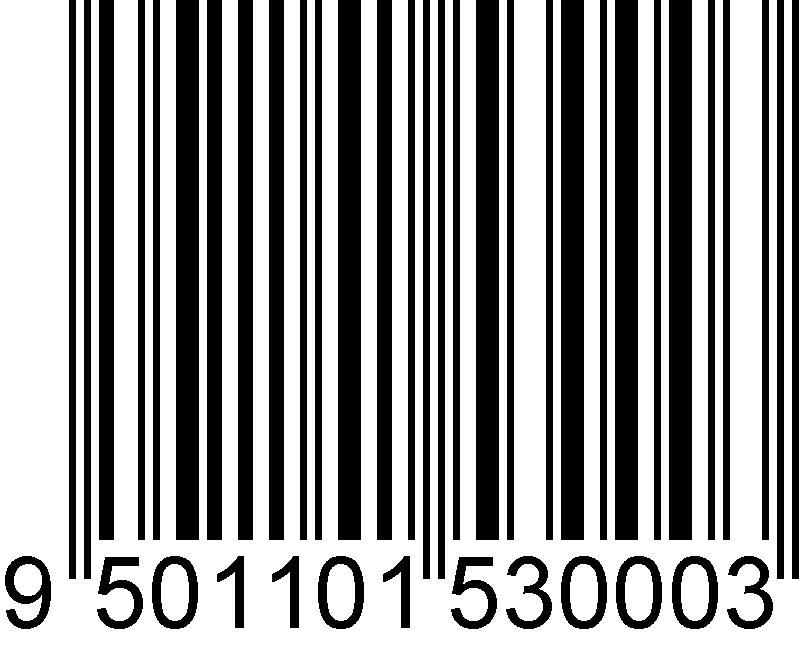
\includegraphics[scale=1.6]{images/barcode.png}
					\caption[Một ví dụ về mã vạch]{Một ví dụ về mã vạch \protect\footnotemark{}}
					\label{fig:barcode}
					\end{figure}
				\footnotetext{\url{http://www.gs1.org/barcodes/ean-upc}}
				\end{itemize}
			\section{Các công cụ sử dụng trong Đề tài}
				\subsection{Môi trường và ngôn ngữ lập trình}
					\begin{itemize}
						\item{\textbf{Môi trường lập trình (IDE):}} trong Đề tài lần này, chúng tôi sử dụng NetBeans để hiện thực hóa ứng dụng của mình vì kích thước của NetBeans không quá lớn, có thể dễ dàng mở rọng với số lượng lớn các module hổ trợ. Ngoài ra, NetBeans IDE là môi trường lập trình mã nguồn mở miễn phí. NetBeans cung cấp cho người dùng các công cụ để viết, biên dịch, gỡ lỗi và triển khai chương trình.
					\begin{figure}[H]
					\centering
					
\includegraphics[scale=0.7]{images/NetBeans.png}
					\caption[Biểu tượng của NetBeans]{Biểu tượng của NetBeans\protect\footnotemark{}}
					\label{fig:NetBeans}
					\end{figure}
					\footnotetext{\url{https://netbeans.org}}
					\item{\textbf{Ngôn ngữ lập trình:}} Java cũng là một ngôn ngữ lập trình mã nguồn mở, hỗ trợ rất nhiều thư viện giúp việc triển khai ứng dụng và thiết kế giao diện. Một số ưu điểm của Java và cũng là lý do mà chúng tôi quyết định sử dụng ngôn ngữ này:
						\begin{itemize}
							\item{Java là một ngôn ngữ lập trình hướng đối tượng. Cú pháp của Java được vay mượn nhiều từ C và C++ nhưng có cú pháp hướng đối tượng đơn giản hơn, ít tính năng xử lý cấp thấp hơn. Do đó, việc viết một chương trình bằng Java dễ dàng, đơn giản hơn và ít tốn công sửa lỗi hơn.}
							\item{Ngoài ra, bộ nhớ trong Java được quản lý và tự động dọn dẹp bằng Java Virtual Machine nên sẽ không có hiện tượng rò rỉ bộ nhớ, rác bộ nhớ. Người lập trình không phải quan tâm đến việc cấp phát và xóa bộ nhớ như C và C++.}
						\end{itemize}
						Chúng tôi sử dụng Java Swing để thiết kế giao diện, Swing hỗ trợ chức năng kéo thả giúp tiện lợi hơn trong việc thiết kế giao diện.
						\begin{figure}[H]
					\centering
					
\includegraphics[scale=0.5]{images/Java.jpg}
					\caption[Biểu tượng của Java]{Biểu tượng của Java \protect\footnotemark{}}
					\label{fig:Java}
					\end{figure}
					\footnotetext{\url{https://java.com}}
					\end{itemize}
				\subsection{Công cụ quản trị cơ sở dữ liệu: MySQL}
					\par MySQL là một hệ quản trị cơ sở dữ liệu quan hệ mã nguồn mở, sử dụng Ngôn ngữ truy vấn có cấu trúc (SQL).
						MySQL có tốc độ xử lý nhanh, ổn định, có tính bảo mật cao và dễ sử dụng. Bên cạnh đó, MySQL có cung cấp phiên bản miễn phí với các tính năng đáp ứng đầy đủ cho việc học tập.
						Với các lý do trên, chúng tôi quyết định sử dụng MySQL để quản lý cơ sở dữ liệu của mình.
							\begin{figure}[H]
								\centering
								
\includegraphics[scale=0.5]{images/mysql.jpg}
								\caption[Biểu tượng của MySQL]{Biểu tượng của MySQL \protect\footnotemark{}}
								\label{fig:mysql}
							\end{figure}
					\footnotetext{\url{https://www.mysql.com/}}
				\subsection{Công cụ khai thác dữ liệu mẫu từ Internet: Selenium}
					\par Selenium là một bộ công cụ giúp tự động hóa trình duyệt web. Selenium có thể chạy trên nhiều hệ điều hành và hỗ trợ nhiều driver cho các trình duyệt khác nhau và được nhiều ngôn ngữ lập trình hỗ trợ, trong đó có Java. \\
					Selenium hoàn toàn miễn phí và không đụng tới vấn đề bản quyền, nên phù hợp với việc nghiên cứu trong học tập.	\\
					Selenium có thể hoạt động một cách tự động được lập trình sẵn, thông qua Selenium, ta có thể lập trình để quy định các hành động sẽ thực thi tự động trên trình duyệt web. \\		
					Ở đề tài này, chúng tôi sử dụng Selenium để tự động hóa việc lấy \textit{(Crawl)} dữ liệu về một số cuốn sách từ các trang web bán sách online (\href{https://tiki.vn}{\textit{tiki.vn}}). Dữ liệu thu được sẽ làm dữ liệu mẫu cho cơ sở dữ liệu của chương trình.
	 						\begin{figure}[H]
								\centering
								
\includegraphics[scale=0.6]{images/selenium.jpg}
								\caption[Selenium và một số browser mà nó hỗ trợ]{Selenium và một số browser mà nó hỗ trợ \protect\footnotemark{}}
								\label{fig:Selenium}
							\end{figure}
							\footnotetext{\url{http://dfinesoft.com/digital-marketing/}}
	\chapter{Phân tích và thiết kế hệ thống}
		\label{system_analysis}	
		\section{Thiết kế hệ thống, cơ sở dữ liệu}			
			\label{database_design}
			\subsection{Một số thông tin về các đặc trưng của hệ thống}
				\begin{itemize}
					\item{Thông tin về tựa sách:} Mỗi tựa sách bao gồm các thông tin sau:
						\begin{itemize}
							\item SKU
							\item Tên sách
							\item Tác giả
							\item Thể loại
							\item Nhà xuất bản
							\item Ngày xuất bản
							\item Giá (Khi thủ thư nhập vào kho)
							\item Số lượng còn lại trong kho
						\end{itemize}
						\item{Thông tin về độc giả:} Mỗi độc giả bao gồm các thông tin sau:
						\begin{itemize}
							\item Mã độc giả
							\item Tên 
							\item Địa chỉ
							\item Ngày sinh
							\item Giới tính
							\item Số CMND
							\item Email
							\item Số điện thoại
						\end{itemize}
						\item{Thông tin về phiếu mượn sách:} 
						\begin{itemize}
							\item Mã độc giả
							\item Mã sách
							\item Ngày mượn
							\item Ngày trả dự kiến
							\item Ngày trả thực tế
						\end{itemize}
				\end{itemize}
			\subsection{Thiết kế cơ sở dữ liệu:}
			Mô hình ER của dữ liệu được mô tả ở \textbf{Hình \ref{fig:er}.}\\
			
			\begin{figure}[h]
			\centering
				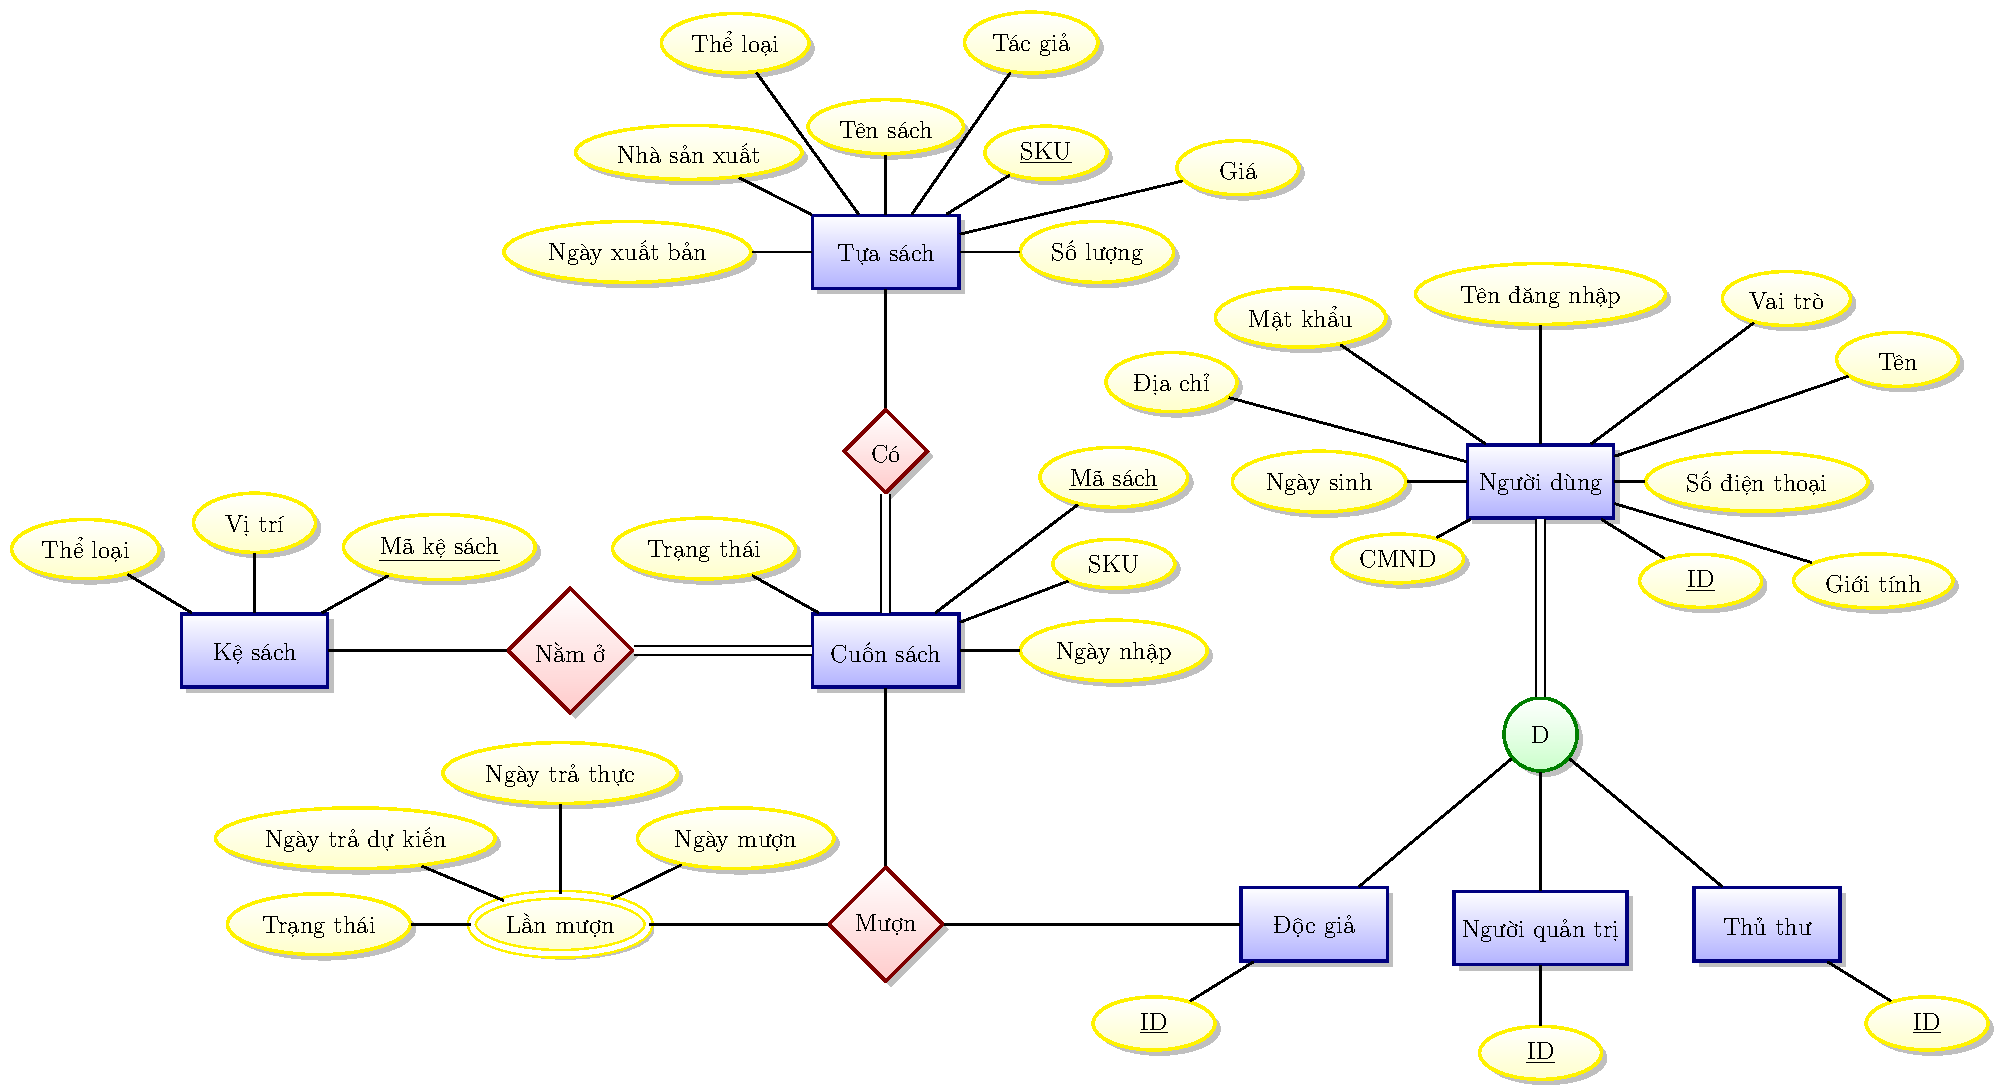
\includegraphics[scale=0.52]{Database.pdf}
				\caption{Mô hình E-R của bài toán}
				\label{fig:er}
			\end{figure}
			
			Trong \textbf{Hình \ref{fig:er}}, có 6 thực thể tham gia vào các mối quan hệ. Trong đó ta quan tâm nhất chủ yếu đến các thực thể \textbf{Tựa sách, Cuốn sách, Độc giả} và mối quan hệ \textbf{Mượn}.
			\par Mỗi tựa sách bao gồm những thông tin mô tả về sách như tên sách hay tác giả,... và phân biệt các tựa sách khác bởi thuộc tính \textit{SKU}. Mỗi tựa sách bao gồm nhiều cuốn sách được đặc trưng bởi thuộc tính \textit{Số lượng}. Mỗi cuốn sách có một \textit{ID} để phân biệt với các cuốn sách khác và người thủ thư trực tiếp quản lý những cuốn sách thay vì từng tựa sách. Một yêu cầu đặt ra cho hệ cơ sở dữ liệu là mỗi khi người thủ thư thêm một cuốn sách của một tựa sách vào thì thuộc tính \textit{Số lượng} sẽ tự động tăng lên một.
			\par Mỗi cuốn sách có một thuộc tính \textit{Trạng thái} để biểu diễn cuốn sách này đang được mượn hay vẫn còn trong thư viện.
			\par Mỗi cuốn sách nằm ở một kệ sách duy nhất, các kệ sách sẽ phân biệt nhau thông qua \textit{Mã kệ sách}, mỗi kệ sách chứa các cuốn sách của một thể loại nhất định. Mỗi kệ sách có thuộc tính \textit{Vị trí} giúp cho việc tìm sách trở nên dễ dàng hơn.
			\par Người dùng được chia ra làm ba loại là: \textbf{Độc giả, Thủ thư. Người quản trị.} Mỗi loại người dùng đều có các thuộc tính như nhau và phân biệt nhau bằng thuộc tính \textit{Vai trò}. Người dùng sẽ được cấp quyền tùy theo vai trò của mình và do đó có những khả năng truy xuất thông tin khác nhau đối với hệ thống.
			\par Mỗi lần độc giả mượn sách, hệ thống sẽ ghi lại ID của độc giả, ID sách mà độc giả đó mượn, ngày mượn, ngày trả dự kiến. Thuộc tính \textit{Trạng thái} trong mối quan hệ \textbf{Mượn} biểu diễn cho việc độc giả đã trả sách hay chưa. Khi độc giả trả sách, hệ thống sẽ cập nhật thêm ngày trả sách thực sự và thuộc tính \textit{Trạng thái} sẽ mang giá trị biểu diễn cho việc độc giả đã trả sách. 
			\subsubsection*{Tạo các bảng trong cơ sở dữ liệu:}
				\begin{itemize}
					\item{Tựa sách được mô tả trong \textbf{Hình \ref{fig:tuasach}}}
					\begin{figure}[H]
						\centering
						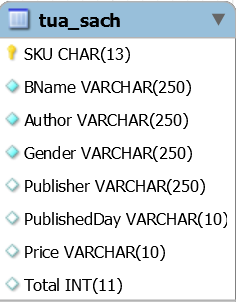
\includegraphics[scale=1]{images/tuasach.png}
						\caption{Thiết kế tựa sách trong CSDL}
						\label{fig:tuasach}
					\end{figure}
					\item{Cuốn sách được mô tả trong \textbf{Hình \ref{fig:cuonsach}}}
					\begin{figure}[H]
						\centering
						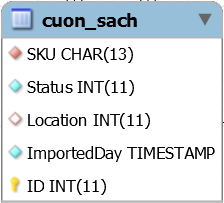
\includegraphics[scale=1]{images/cuonsach.png}
						\caption{Thiết kế cuốn sách trong CSDL}
						\label{fig:cuonsach}
					\end{figure}
					\item{Kệ sách được mô tả trong \textbf{Hình \ref{fig:kesach}}}
					\begin{figure}[H]
						\centering
						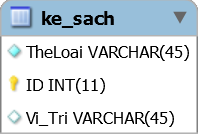
\includegraphics[scale=1]{images/kesach.png}
						\caption{Kệ sách được mô tả trong MySQL}
						\label{fig:kesach}
					\end{figure}
					\item{Độc giả được mô tả trong \textbf{Hình \ref{fig:docgia}}}
					\begin{figure}[H]
						\centering
						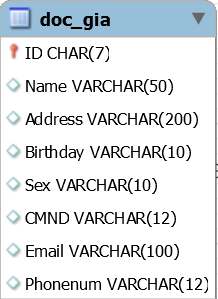
\includegraphics[scale=1]{images/docgia.png}
						\caption{Thông tin về độc giả trong CSDL}
						\label{fig:docgia}
					\end{figure}
					\item{Lần mượn sách được mô tả trong \textbf{Hình \ref{fig:muon}}}
					\begin{figure}[H]
						\centering
						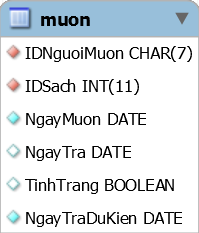
\includegraphics[scale=1]{images/muon.png}
						\caption{Thông tin mỗi lần mượn sách trong CSDL}
						\label{fig:muon}
					\end{figure}
				\end{itemize}
		\subsection{Các chức năng chính của hệ thống}
			\begin{itemize}
				
				\item Chức năng của khách
					\begin{itemize}
						\item Tra cứu thông tin sách
						\item Đăng nhập vào hệ thống
						\item Đăng ký tài khoản
					\end{itemize}
				\item Chức năng của người quản trị hệ thống:
					\begin{itemize}
						\item Quản lý thủ thư, thêm, xóa và cập nhật thông tin thủ thư
						\item Quản lý độc giả, thêm, xóa và cập nhật thông tin độc giả
						\item Sao lưu và phục hồi dữ liệu
					\end{itemize}
				\item Chức năng của thủ thư:
				\begin{itemize}
					\item Quản lý cuốn sách
					\begin{itemize}
						\item Tra cứu, tìm kiếm sách hiện có
						\item Thêm, cập nhật, xóa một tựa sách, cuốn sách
					\end{itemize}
				\item Quản lý độc giả
					\begin{itemize}
						\item Xem danh sách độc giả
					\end{itemize}
				\item Quản lý thông tin mượn-trả sách
					\begin{itemize}
						\item Xem thông tin mượn-trả sách 
						\item Cập nhật thông tin mượn-trả sách
						\item Cập nhật thông tin sách đến hạn trả
					\end{itemize}
				\item Tổng hợp báo cáo hàng tháng
				\end{itemize}
				\item Chức năng của độc giả:
					\begin{itemize}
						\item Xem, cập nhật thông tin
						\item Tra cứu danh sách mượn-trả
						\item Tìm kiếm, xem thông tin sách
					\end{itemize}
			\end{itemize}
		\subsection{Sơ đồ phân cấp các chức năng của ứng dụng:}
			\begin{figure}[H]
				\centering
				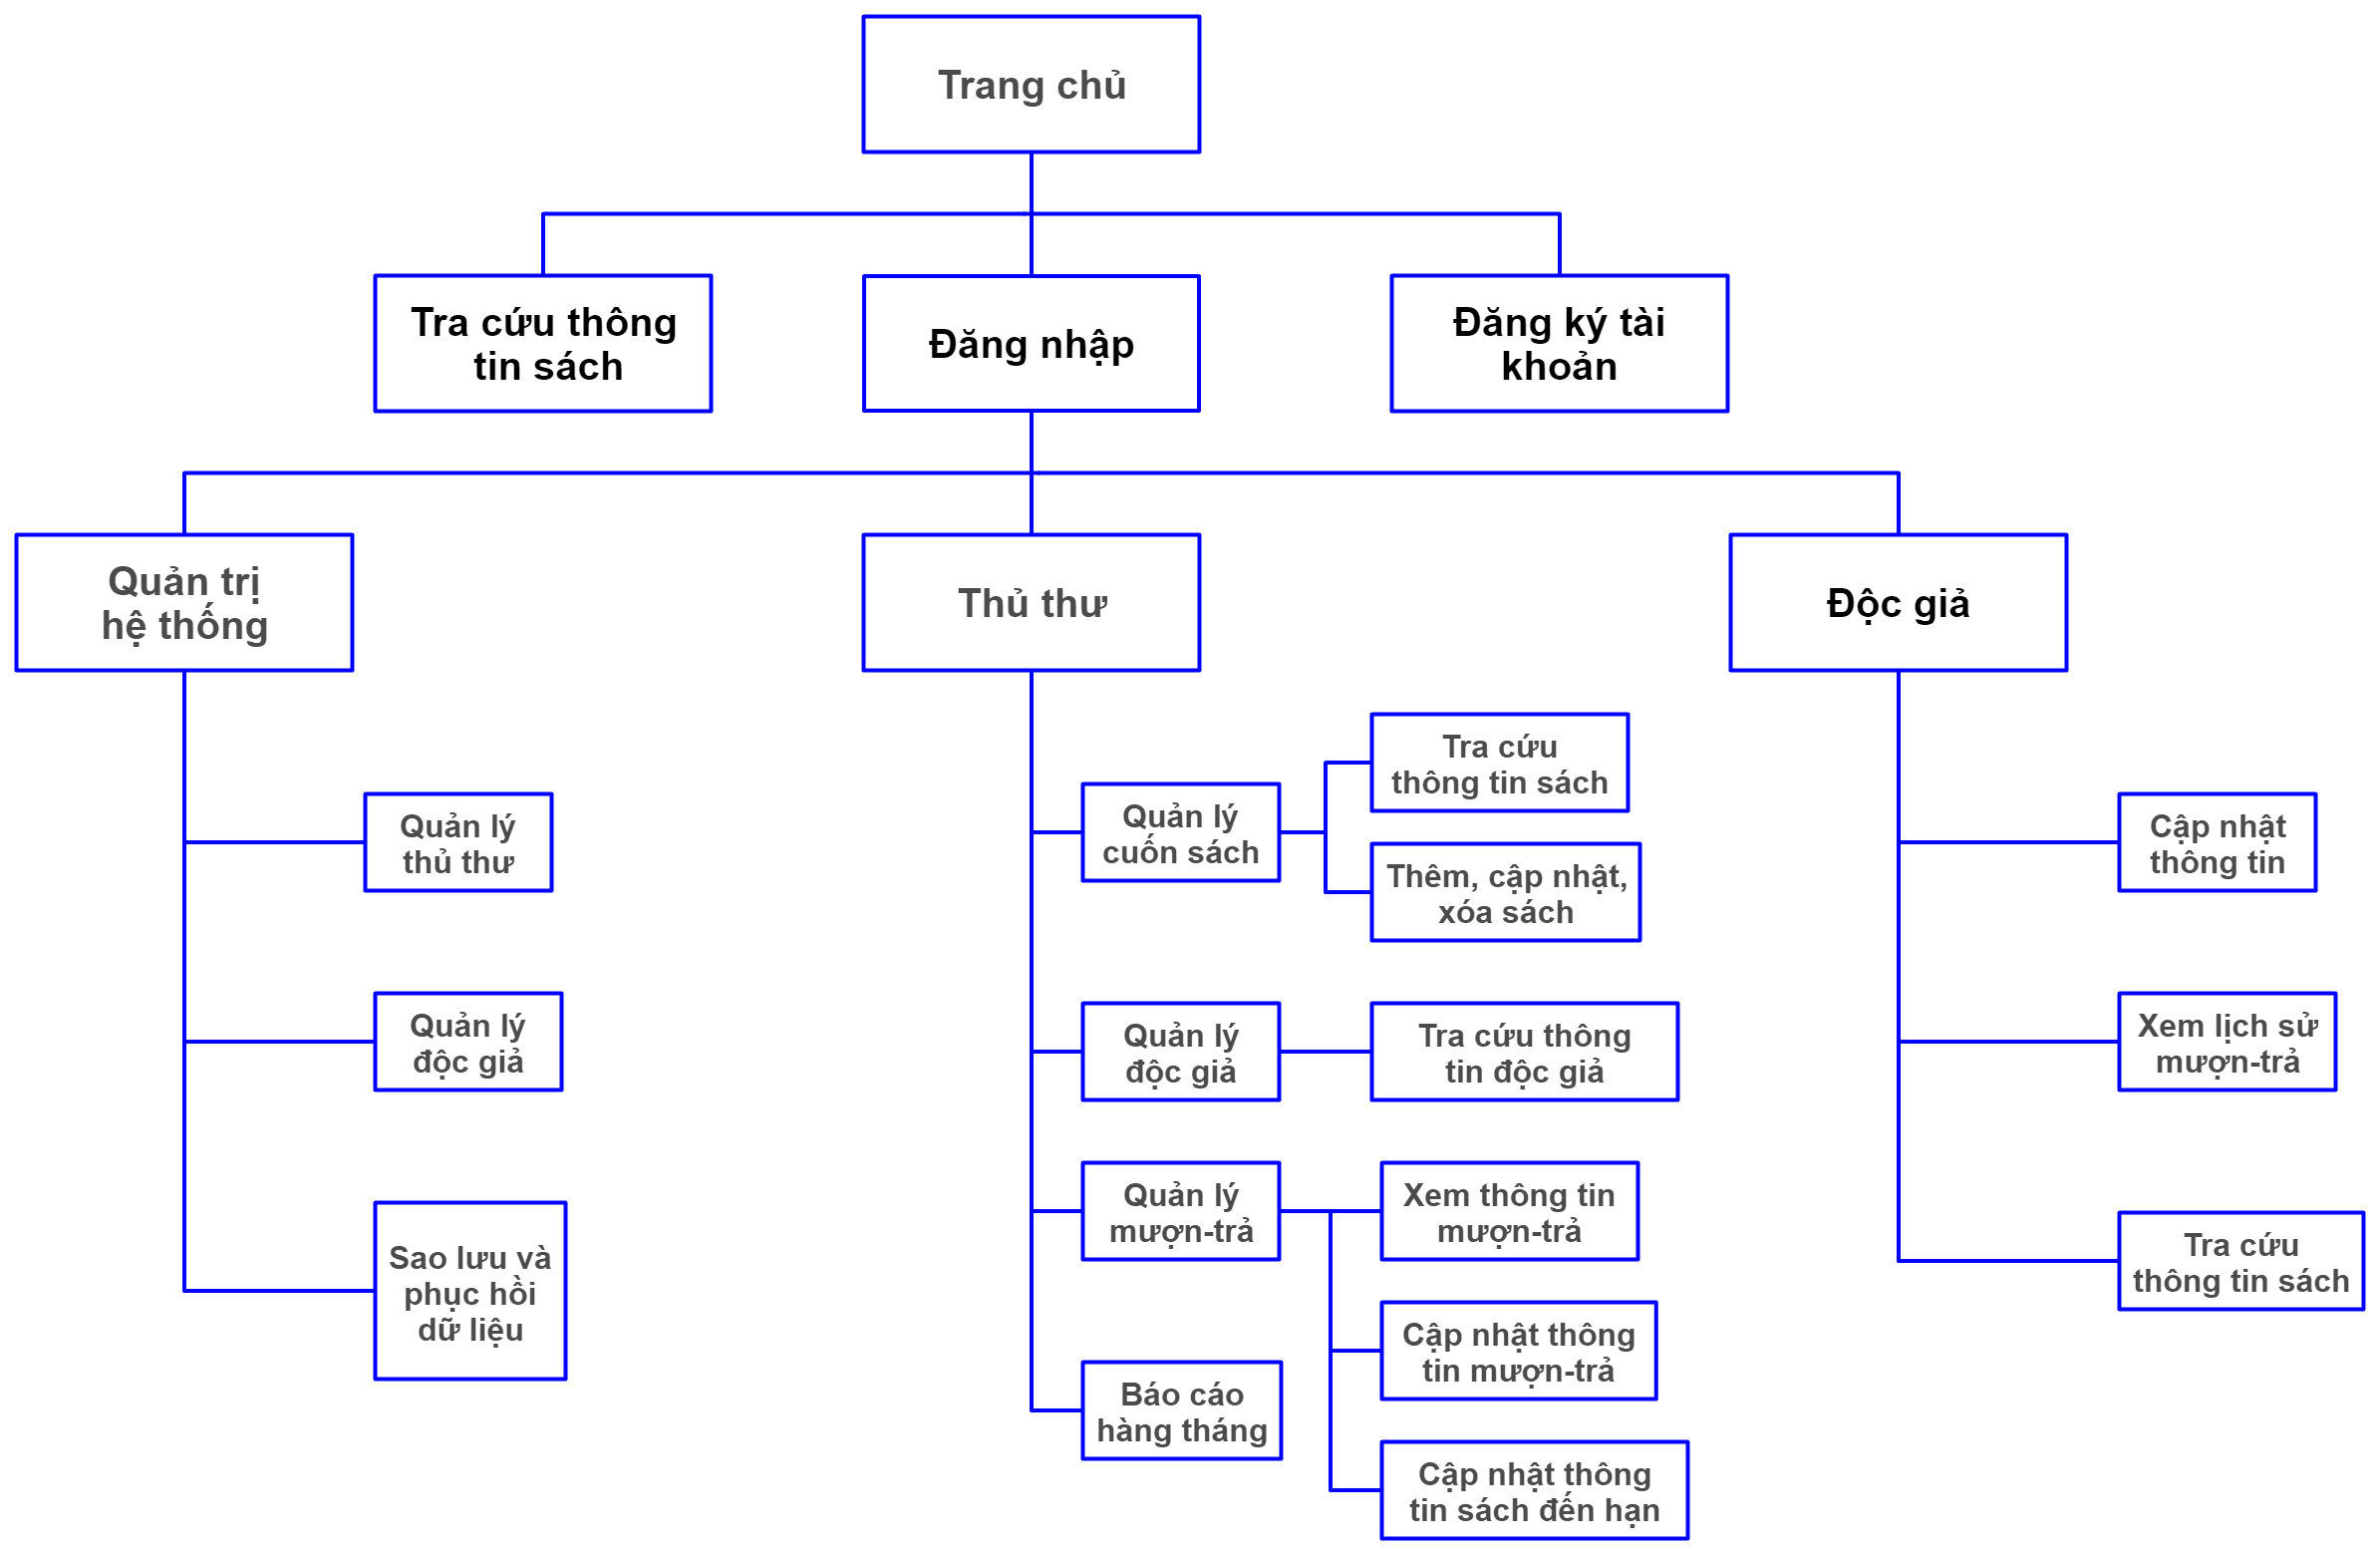
\includegraphics[scale=0.25]{images/TFHD.png}
				\caption{Sơ đồ phân cấp chức năng}
				\label{fig:tfhd}
			\end{figure}
	\chapter{Sản phẩm cuối cùng}
				\section{Khởi động hệ thống}
					\begin{figure}[H]
						\centering
						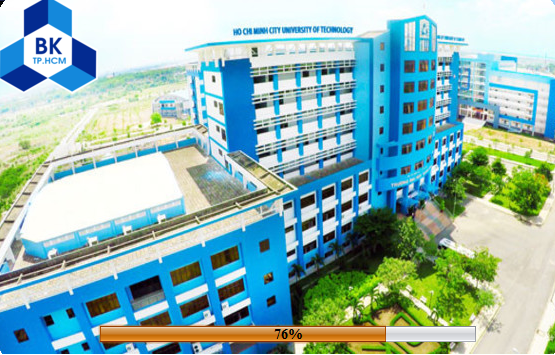
\includegraphics[scale=0.8]{images/startup.png}
						\caption{Khởi động ứng dụng}
						\label{fig:startup}
					\end{figure}
				\section{Màn hình chính} 
					Trang màn hình chính của ứng dụng hiện ra như trong \textbf{Hình \ref{fig:mainscreen}}.\\
					\begin{figure}
						\centering
						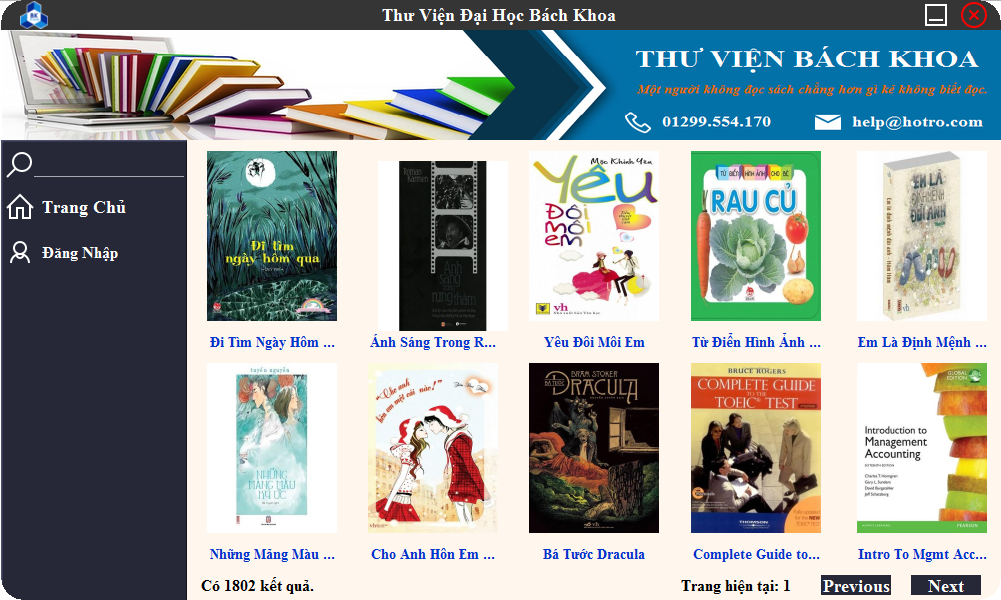
\includegraphics[scale=0.65]{images/mainscreen.png}
						\caption{Màn hình chính của ứng dụng}
						\label{fig:mainscreen}
					\end{figure}
					Giao diện màn hình chính này cung cấp 2 chức năng cho người sử dụng.
					\begin{itemize}
						\item Người dùng có thể tìm những cuốn sách có trong thư viện, xem các thông tin của sách. Mặc định từ khóa tìm kiếm sẽ liên quan đến: \textit{Tên, Tác giả, Thể Loại, Nhà xuất bản}. Vì vậy tất cả các cuốn sách có liên quan sẽ được hiển thị và số lượng kết quả tìm được cũng được hiển thị. 
						Một ví dụ về thông tin sách được mô tả ở \textbf{Hình \ref{fig:example}}
						\begin{figure}
						\centering
						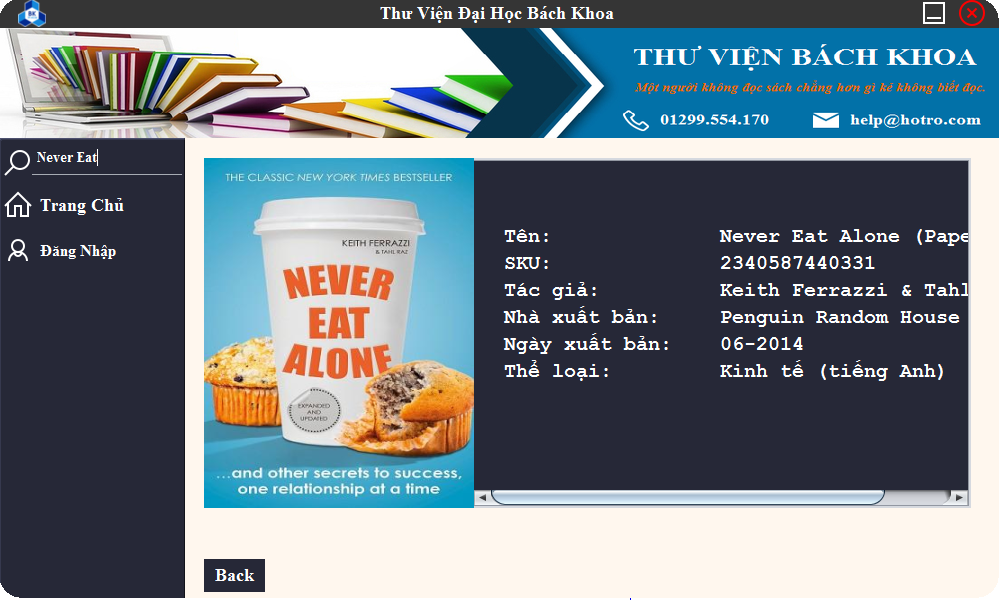
\includegraphics[scale=0.65]{images/example.png}
						\caption{Thông tin một quyển sách đươc hiển thị trong ứng dụng}
						\label{fig:example}
						\end{figure}
						\item Chức năng thứ hai là chức năng đăng nhập. Chức năng này giúp người sử dụng đăng nhập vào tài khoản của mình. Và như đã mô tả trong \textbf{Hình \ref{fig:tfhd}}, tùy theo vai trò \textit{Độc giả, Thủ thư, Người quản trị} mà các giao diện chức năng của các người dùng sẽ khác nhau.\\
						Việc đăng nhập cũng trở nên dễ dàng hơn khi có thêm chức năng \textit{Đăng nhập bằng thẻ}. Người dùng chỉ cần Scan mã vạch của mình để đăng nhập vào hệ thống. Màn hình đăng nhập được mô tả trong \textbf{Hình \ref{fig:signin}}\\
						\begin{figure}
						\centering
						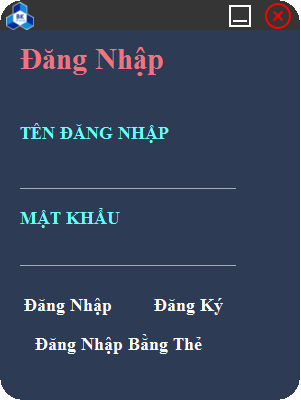
\includegraphics[scale=0.75]{images/signin.png}
						\caption{Màn hình đăng nhập}
						\label{fig:signin}
						\end{figure}
						Ngoài ra nếu một độc giả chưa có tài khoản, có thể tự đăng ký với chức năng đăng ký tài khoản của ứng dụng, chức năng này được mô tả trong \textbf{Hình \ref{fig:signup}}
						\begin{figure}
						\centering
						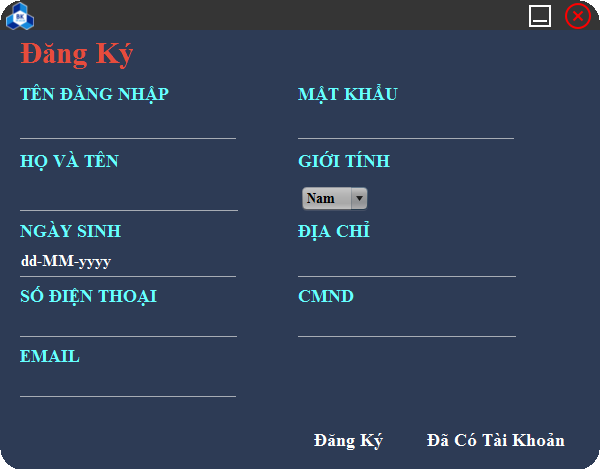
\includegraphics[scale=0.75]{images/signup.png}
						\caption{Màn hình đăng ký tài khoản}
						\label{fig:signup}
						\end{figure}
					\end{itemize}
				\section{Giao diện người quản trị hệ thống} 
				Như đã trình bày ở \textit{Sơ đồ phân cấp các chức năng của ứng dụng} ở \textbf{Hình \ref{fig:tfhd}}, người quản trị hệ thống có 3 chức năng chính đó là \textit{Quản lý thủ thư, Quản lý độc giả, Sao lưu và khôi phục dữ liệu}.\\
				
				\begin{itemize}
					\item Quản lý thủ thư\\
					Ứng dụng cung cấp cho người quản trị hệ thống những chức năng như: Tìm kiếm, liệt kê danh sách thủ thư, thêm một thử thư, chỉnh sửa, thay đổi thông tin thủ thư. Một số hình ảnh về giao diện quản lý thủ thư như trong \textbf{Hình \ref{fig:lib1}, Hình \ref{fig:lib2}, Hình \ref{fig:lib3}}
					\begin{figure}
						\centering
						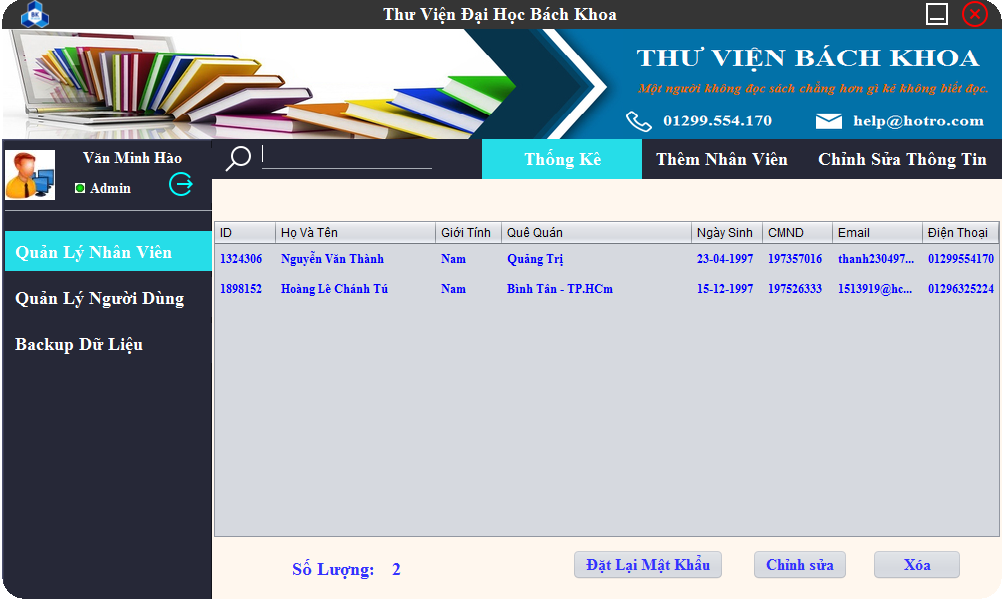
\includegraphics[scale=0.65]{images/lib1.png}
						\caption{Liệt kê danh sách thủ thư}
						\label{fig:lib1}
						\end{figure}
						
						\begin{figure}
						\centering
						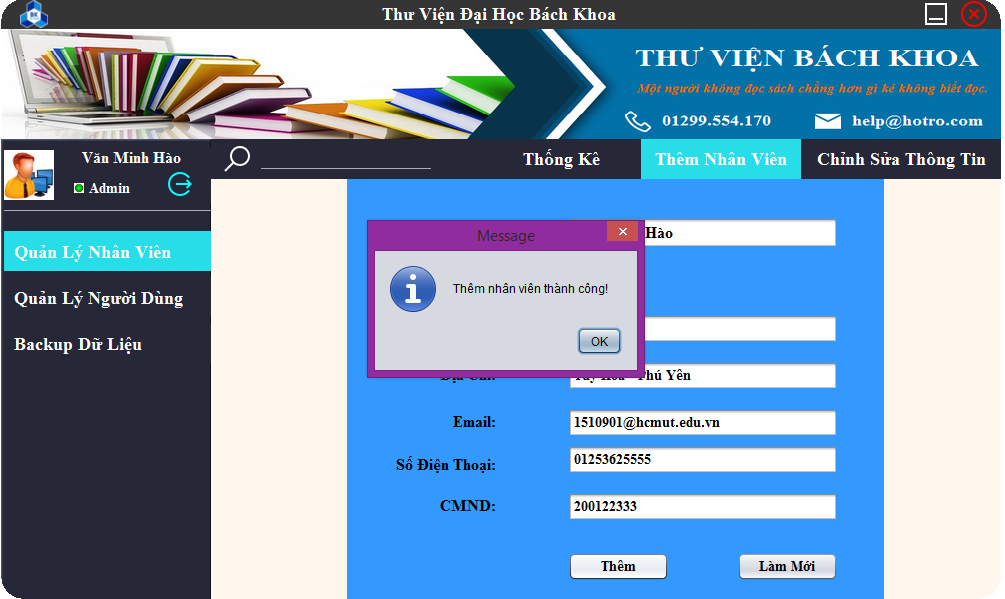
\includegraphics[scale=0.65]{images/lib2.png}
						\caption{Thêm thủ thư}
						\label{fig:lib2}
						\end{figure}
						
						\begin{figure}
						\centering
						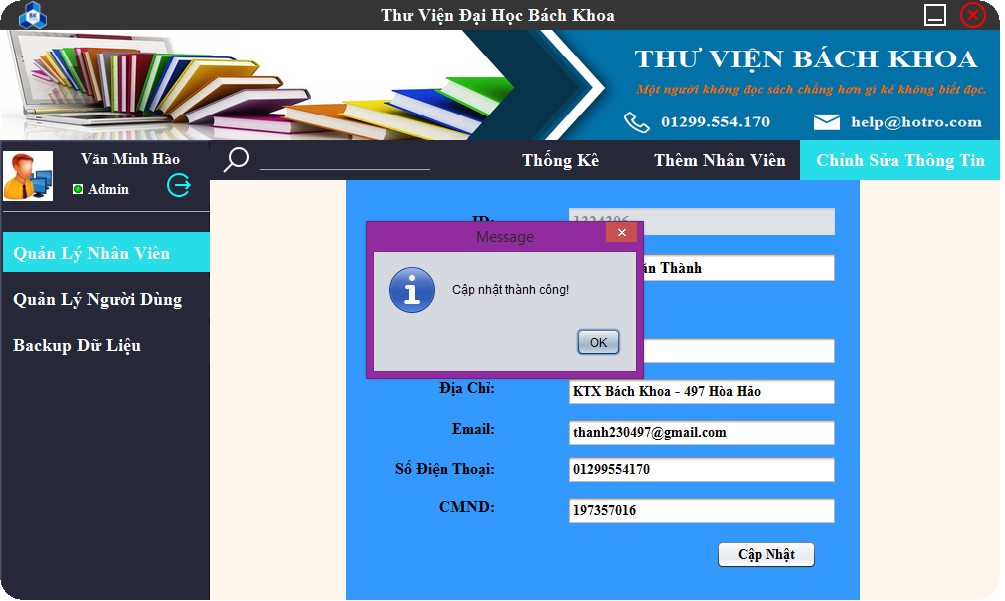
\includegraphics[scale=0.65]{images/lib3.png}
						\caption{Chỉnh sửa thông tin thủ thư}
						\label{fig:lib3}
						\end{figure}
					\item Quản lý độc giả\\
					Về cơ bản, các chức năng quản lý thủ thư và quản lý độc giả là như nhau. \textbf{Hình \ref{fig:reader}} mô tả chức năng quản lý độc giả.
					\begin{figure}
						\centering
						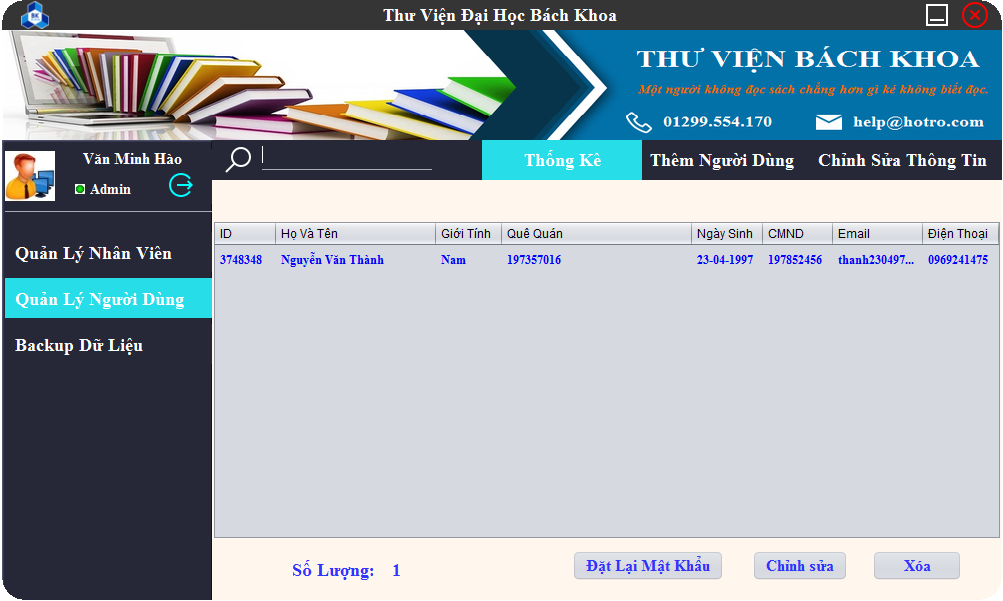
\includegraphics[scale=0.65]{images/reader1.png}
						\caption{Thống kê độc giả}
						\label{fig:reader}
						\end{figure}
					
					\item Sao lưu và phục hồi dữ liệu\\
					Ngoài hai chức năng cơ bản trên, người quản trị hệ thống còn phải có khả năng sao lưu và phục hồi dữ liệu phòng khi có sự cố xảy ra. Giao diện chức năng này được mô tả trong \textbf{Hình \ref{fig:backup}}
					
						\begin{figure}[H]
						\centering
						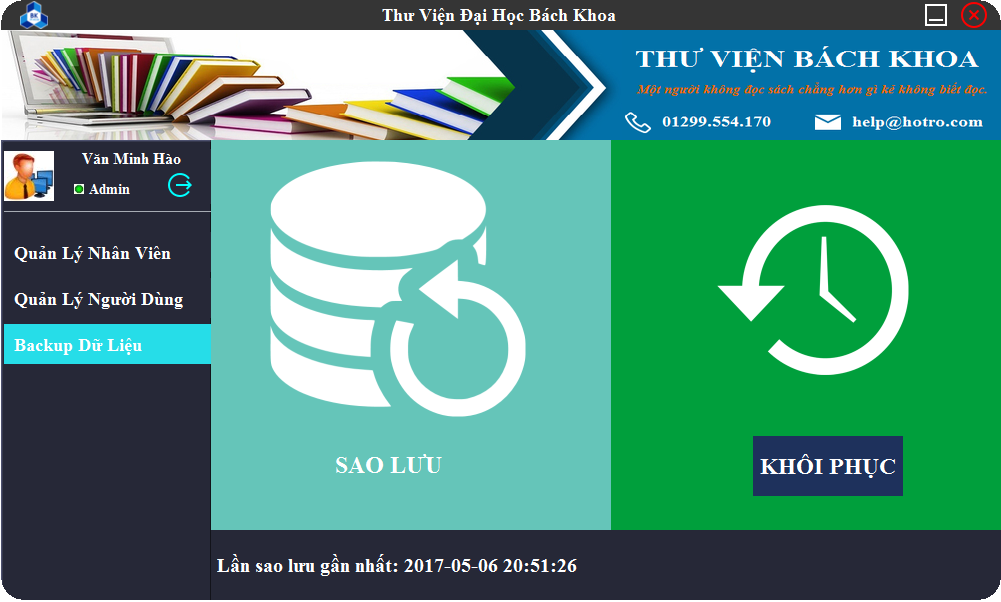
\includegraphics[scale=0.6]{images/backup.png}
						\caption{Sao lưu và phục hồi dữ liệu}
						\label{fig:backup}
						\end{figure}			
				\end{itemize}
			\section{Giao diện của độc giả}
			Ứng dụng cung cấp cho độc giả các chức năng về quản lý tài khoản, thay đổi thông tin tài khoản của mình, tìm kiếm thông tin sách và các lần mượn sách của mình.\\
			Ngoài cách tìm kiếm thông thường, ứng dụng cung cấp cho độc giả tìm kiếm nâng cao với sự lựa chọn các trường(\textit{field}) muốn tìm kiếm giúp cho việc tìm kiếm trở nên dễ dàng hợn.
			Dưới đây là một số hình ảnh về giao diện của độc giả có trong ứng dụng (\textbf{Hình \ref{fig:rdsearch}, Hình \ref{fig:readerinfor}})
						\begin{figure}[H]
						\centering
						\includegraphics[scale=0.65]{images/searchreader.png}
						\caption{Chức năng tìm kiếm sách của độc giả}
						\label{fig:rdsearch}
						\end{figure}
						
						\begin{figure}
						\centering
						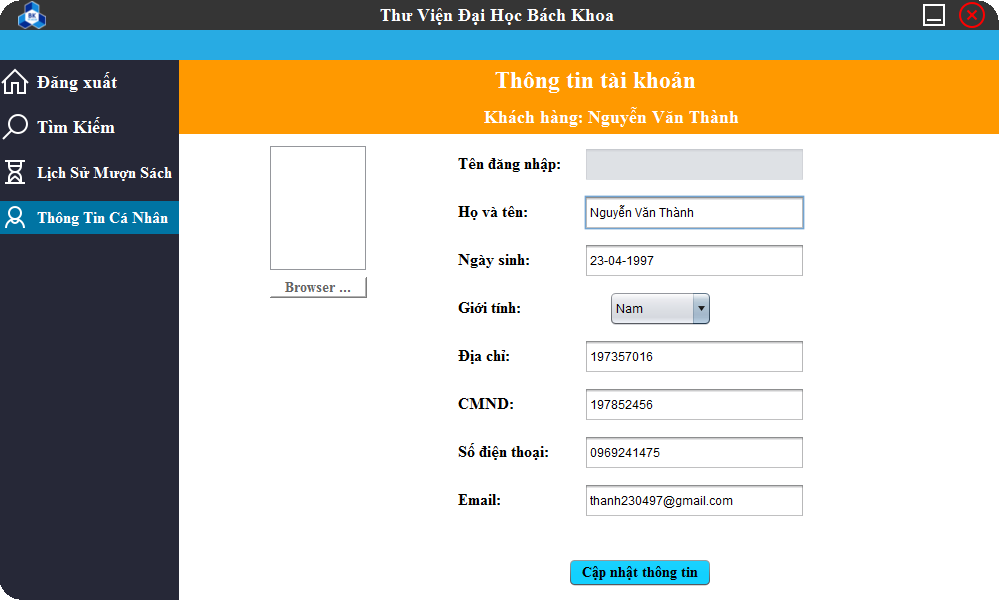
\includegraphics[scale=0.65]{images/inforreader.png}
						\caption{Chức năng xem và chỉnh sửa thông tin cá nhân của độc giả}
						\label{fig:readerinfor}
						\end{figure}
			\section{Giao diện của thủ thư}
			Ứng dụng cung cấp cho người thủ thư các chức năng về tìm kiếm, cập nhật thông tin sách, thêm, xóa sách trong thư viện và thống kê việc mượn trả sách của độc giả cũng như thống kê kho sách.\\
			Ứng dụng cung cấp cho người thủ thư chức năng tìm kiếm sách nâng cao. Sau khi tìm kiếm sách có thể nhấp xem thông tin sách và cập nhật thông tin cuốn sách đó.\\
			Thủ thư có thể lấy thống kê tình trạng kho sách để đưa ra báo cáo hàng tháng.\\
			Chức năng quản lý độc giả gồm tình trạng mượn, trả sách của các độc giả và sử dụng mã vạch để thực hiện mượn trả sách trực tiếp.\\
			Dưới đây là một số hình ảnh về giao diện của thủ thư có trong ứng dụng (\textbf{Hình \ref{fig:mgrsearch}, Hình \ref{fig:mgrbookinfor}, Hình \ref{fig:mgrupdatebook}, Hình \ref{fig:mgruserstats1}, Hình \ref{fig:mgruserstats2}, Hình \ref{fig:mgrborrowbook}, Hình \ref{fig:mgrstoragestats}})
						\begin{figure}
						\centering
						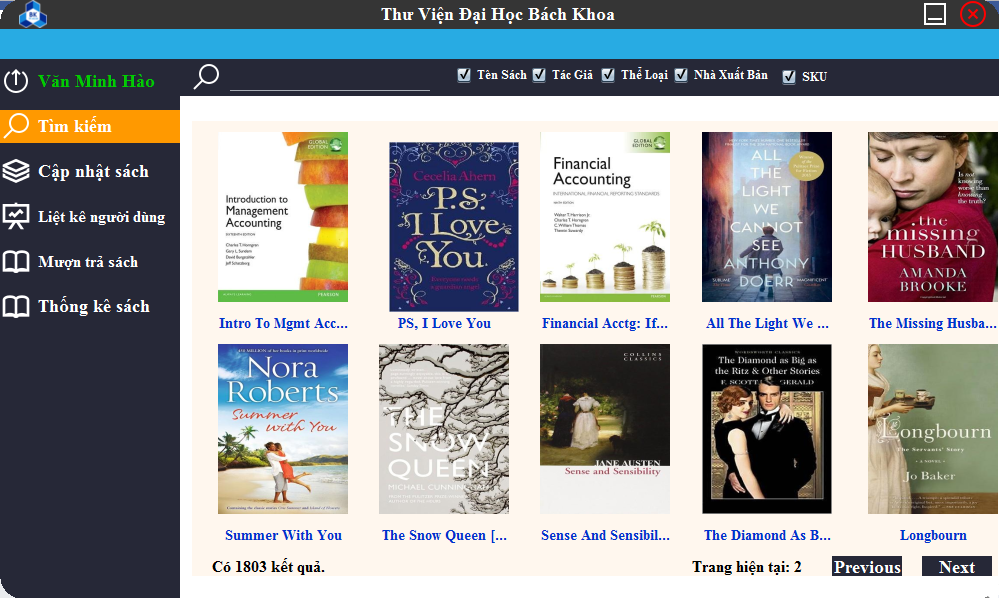
\includegraphics[scale=0.65]{images/mgr1.png}
						\caption{Chức năng tìm kiếm sách của thủ thư}
						\label{fig:mgrsearch}
						\end{figure}
						
						\begin{figure}
						\centering
						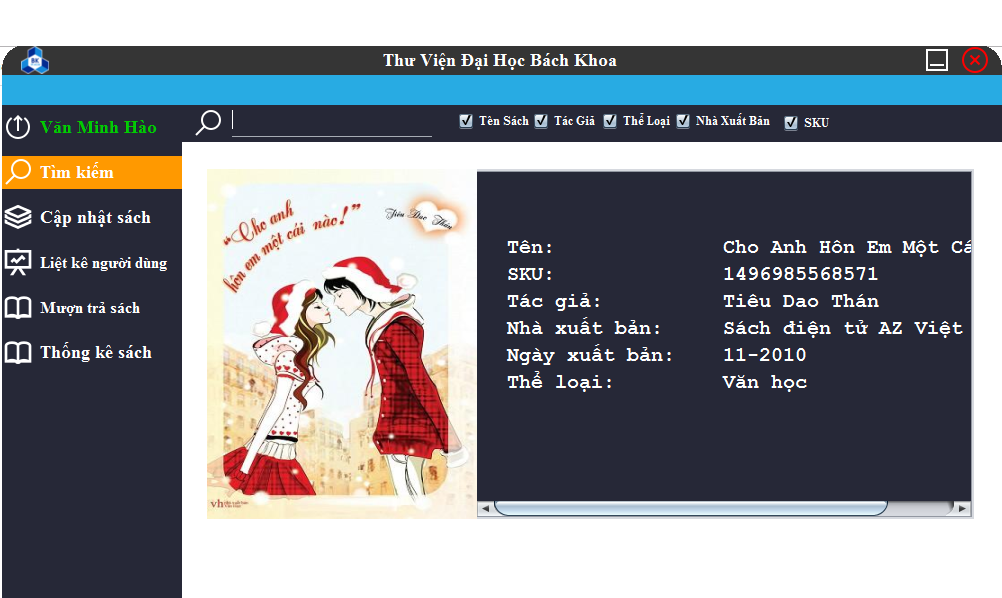
\includegraphics[scale=0.65]{images/mgr2.png}
						\caption{Xem thông tin chi tiết sách sau khi tìm kiếm}
						\label{fig:mgrbookinfor}
						\end{figure}
						
						\begin{figure}
						\centering
						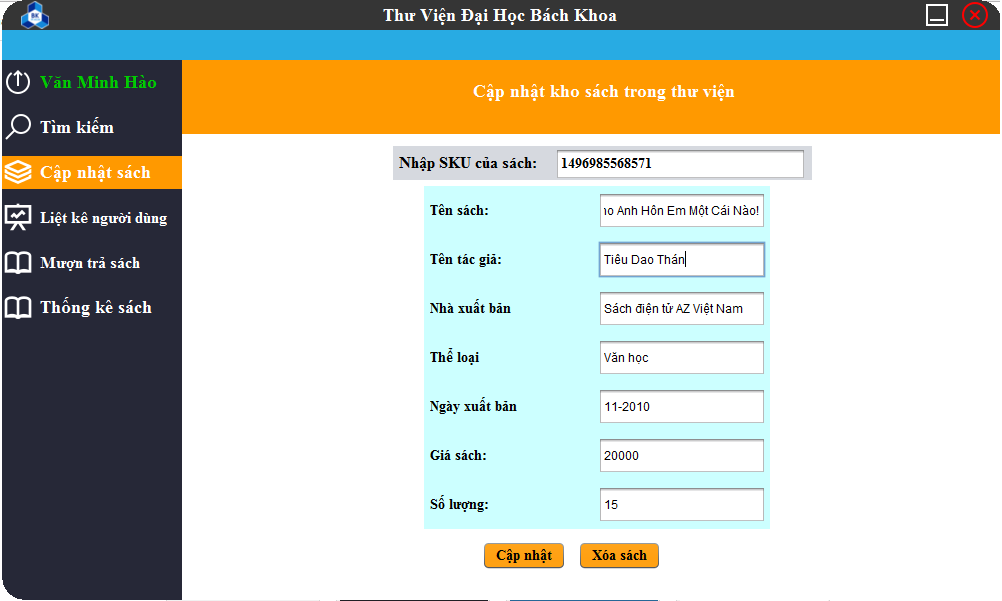
\includegraphics[scale=0.65]{images/mgr3.png}
						\caption{Chức năng thêm, xóa, cập nhật thông tin sách}
						\label{fig:mgrupdatebook}
						\end{figure}
						
						\begin{figure}
						\centering
						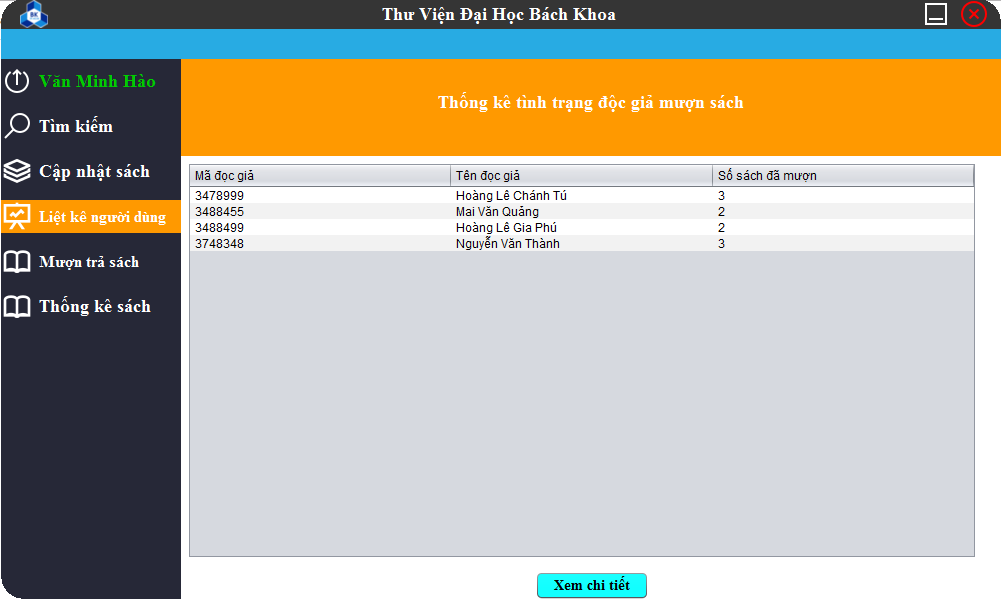
\includegraphics[scale=0.65]{images/mgr4.png}
						\caption{Chức năng liệt kê các độc giả và thông tin cơ bản}
						\label{fig:mgruserstats1}
						\end{figure}
						
						\begin{figure}
						\centering
						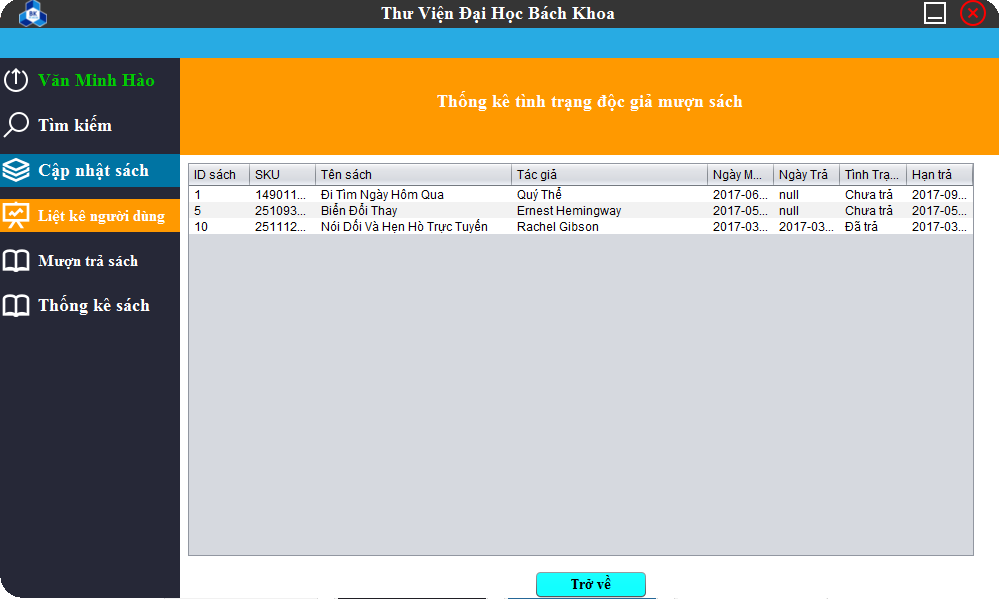
\includegraphics[scale=0.65]{images/mgr5.png}
						\caption{Lịch sử mượn, trả sách của một độc giả}
						\label{fig:mgruserstats2}
						\end{figure}
						
						\begin{figure}
						\centering
						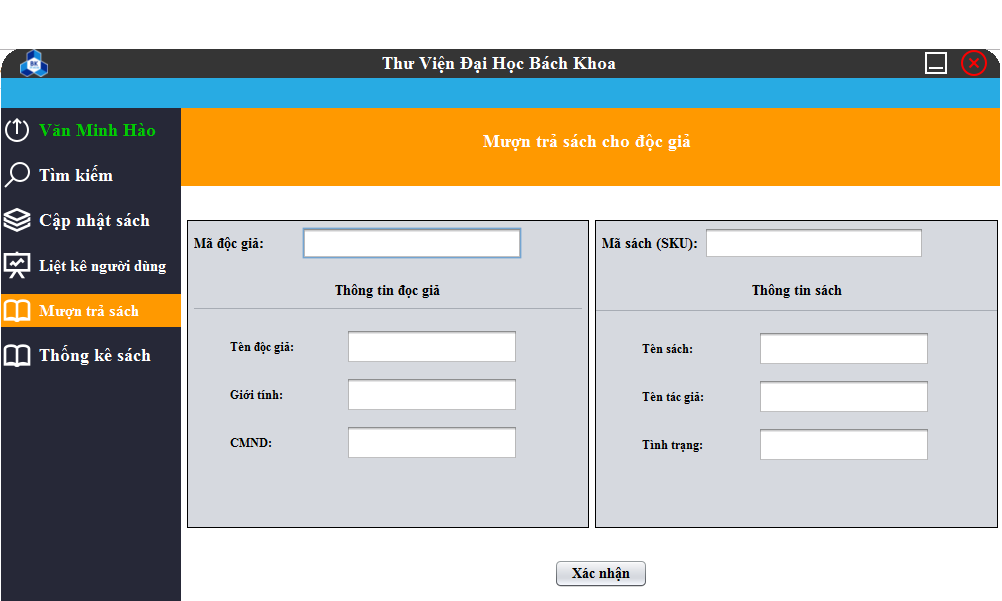
\includegraphics[scale=0.65]{images/mgr6.png}
						\caption{Chức năng mượn trả sách bằng sử dụng mã vạch}
						\label{fig:mgrborrowbook}
						\end{figure}
						
						\begin{figure}
						\centering
						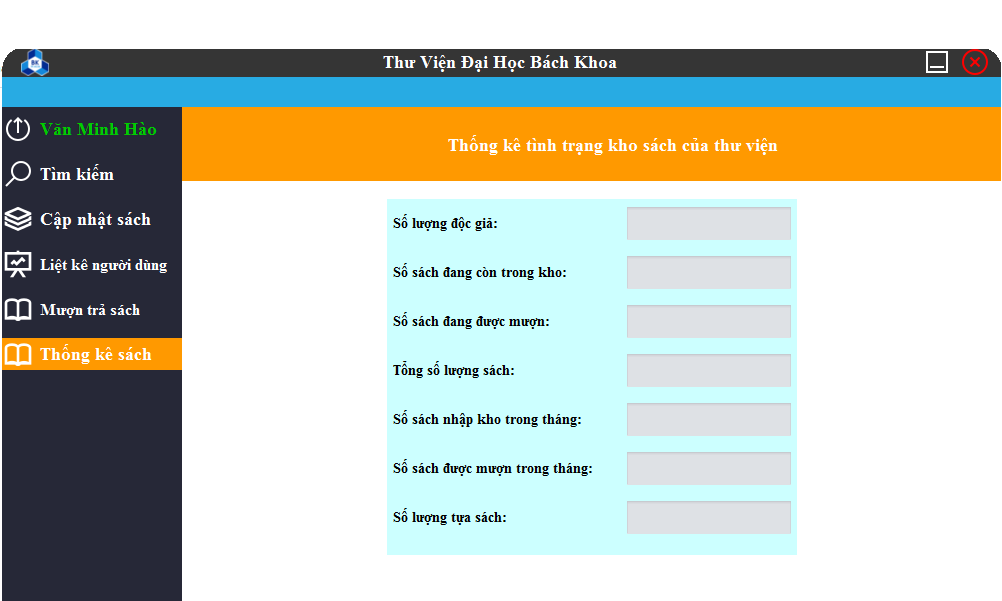
\includegraphics[scale=0.65]{images/mgr7.png}
						\caption{Thống kê tình trạng kho sách của thư viện}
						\label{fig:mgrstoragestats}
						\end{figure}
	\chapter{Tổng kết}
		\section{Kết quả đạt được}
			\begin{itemize}
				\item Về mặt sản phẩm, chúng tôi đã thiết kế được một CSDL và tạo ra một phần mềm giao diện người dùng phù hơp với chức năng của một phần mềm quản lý Thư viện. Sản phẩm dễ sử dụng, thân thiện với người dùng, nhận được một số phản hồi khá tích cực.
			\end{itemize}
		\section{Khó khăn và hạn chế}
			\begin{itemize}
				\item Những yêu cầu ban đầu mà nhóm đặt ra thực sự vượt quá sức của các thành viên trong nhóm do sự hạn chế về kiến thức và kinh nghiệm. Tuy nhiên, tất cả các thành viên trong nhóm đã làm việc rất tích cực, chuyên nghiệp. Mọi người hoàn thành tốt phân việc của mình, và sau dự án này, mọi người đã học hỏi được nhiều điều về kỹ năng làm việc nhóm.
				\item Java là một ngôn ngữ mới đối với tất cả thành viên trong nhóm, vì vậy trong quá trình thiết kế giao diện, nhóm gặp khá nhiều những khó khăn trong việc tìm và sửa lỗi. Phải mất một khoảng thời gian tìm hiểu, nhóm mới làm quen được với ngôn ngữ này.
				\item Thiết kế được một CSDL tốt luôn luôn là một công việc khó, vì vậy CSDL của chúng tôi chưa đáp ứng được những chức năng, yêu cầu cao. 
				\item Sản phẩm chưa được kiểm thử chặt chẽ nên vẫn còn một số lỗi.
				\item Sự xuất của mã vạch(\textit{barcode}) trong ứng dụng chưa nhiều, chưa đạt được yêu cầu đề ra của cả nhóm lúc bắt đầu dự án.
				\item Sản phẩm chưa có chức năng toàn màn hình(\textit{Full Screen}.
			\end{itemize}
		\section{Hướng phát triển trong tương lai}
			\begin{itemize}
				\item Trong tương lai, nếu có cơ hội, nhóm sẽ khắc phục những lỗi mà sản phẩm hiện tại còn mắc phải.
				\item Nghiên cứu sâu về mã vạch và ứng dụng sâu hơn vào việc quản lý Thư viện
				\item Phát triển ứng dụng trên một số hệ điều hành khác như \textbf{Linux, Mac OS}.
				\item Phát triển chức năng toàn màn hình cho ứng dụng.
				\item Phát triển ứng dụng với khả năng quản lý kho dữ liệu lớn hơn(hơn 100.000 sách).
			\end{itemize}
	\newpage
	\section*{Phân chia công việc}
	\addcontentsline{toc}{chapter}{Phân chia công việc}
			\addcontentsline{lof}{section}{Phân chia công việc}
			\begin{figure}[H]
				\centering
				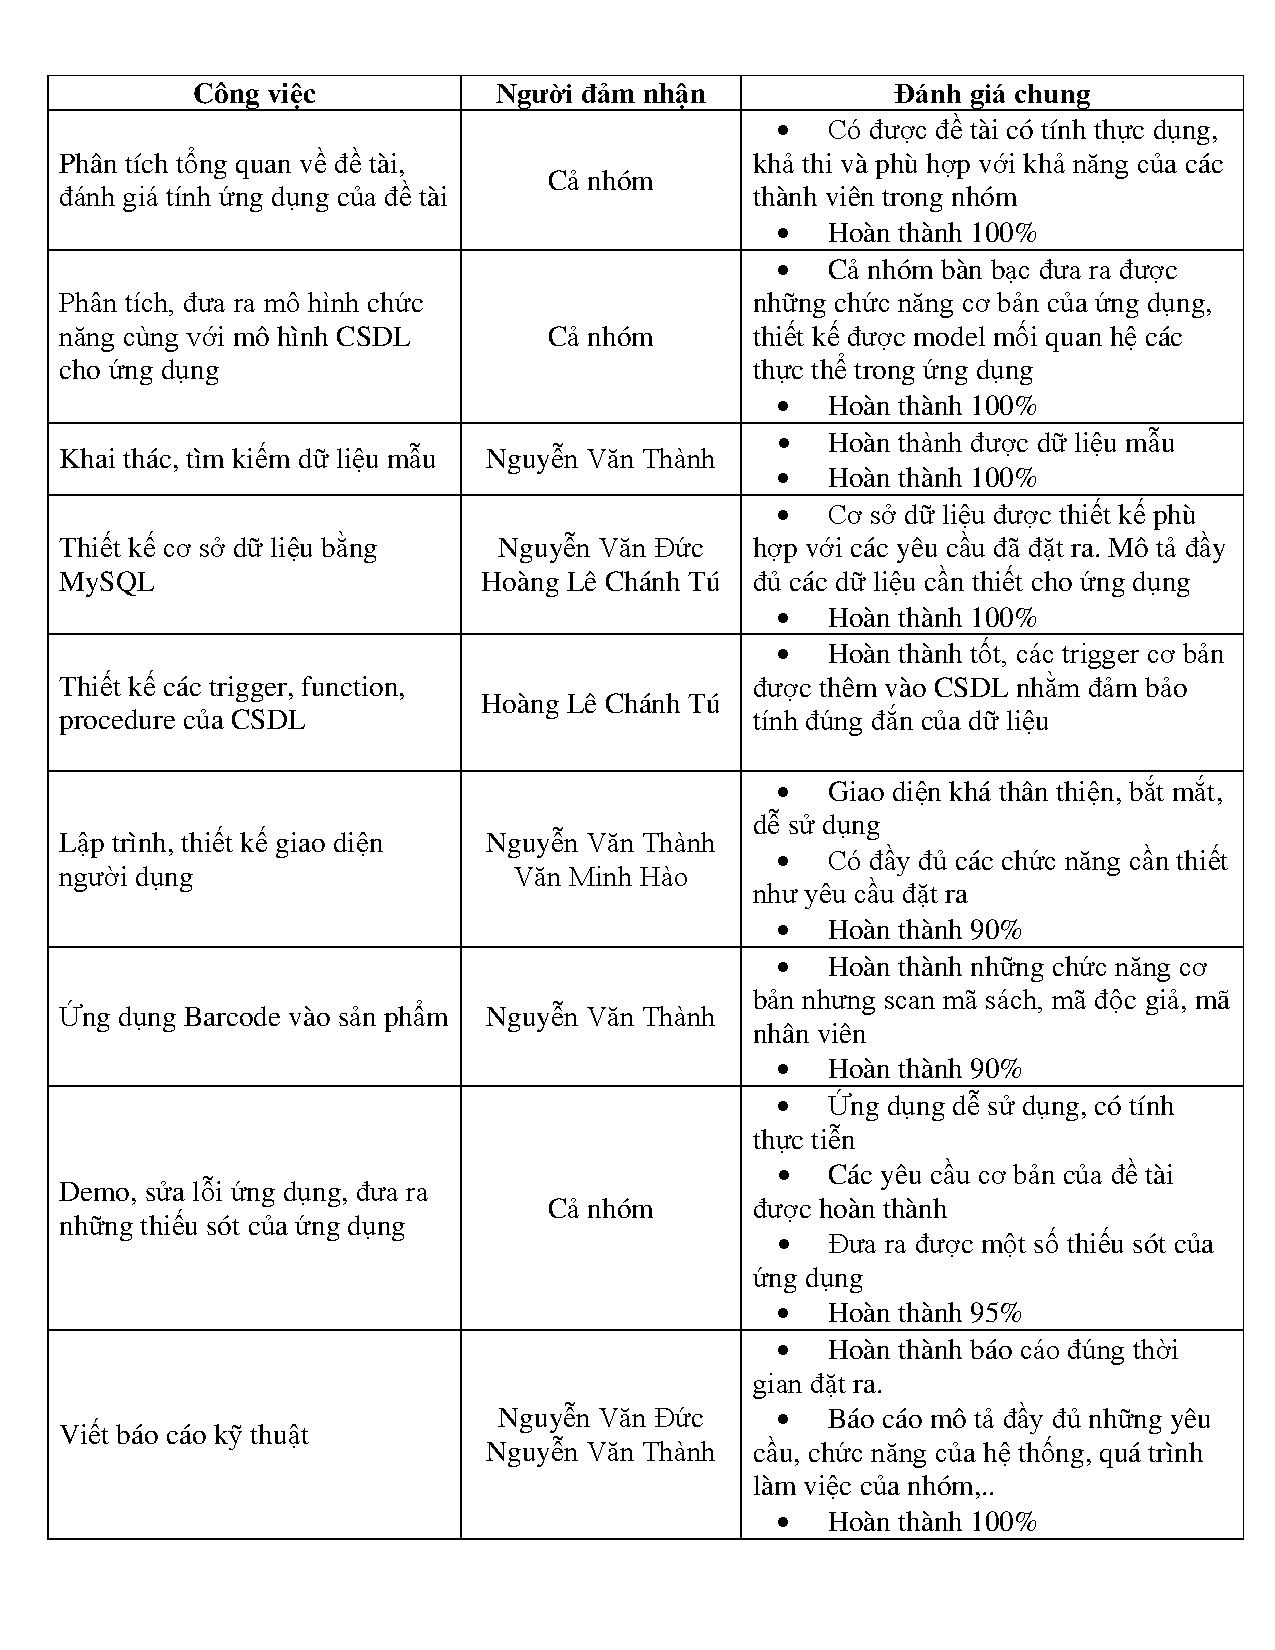
\includegraphics[scale=0.8]{images/phanchiacongviec.pdf}
				\label{fig:work}
			\end{figure}
	\newpage
	\section*{Biên bản họp nhóm}
	\addcontentsline{toc}{chapter}{Biên bản họp nhóm}
			\addcontentsline{lof}{section}{Lần họp thứ nhất}
			\begin{figure}[H]
			\centering
			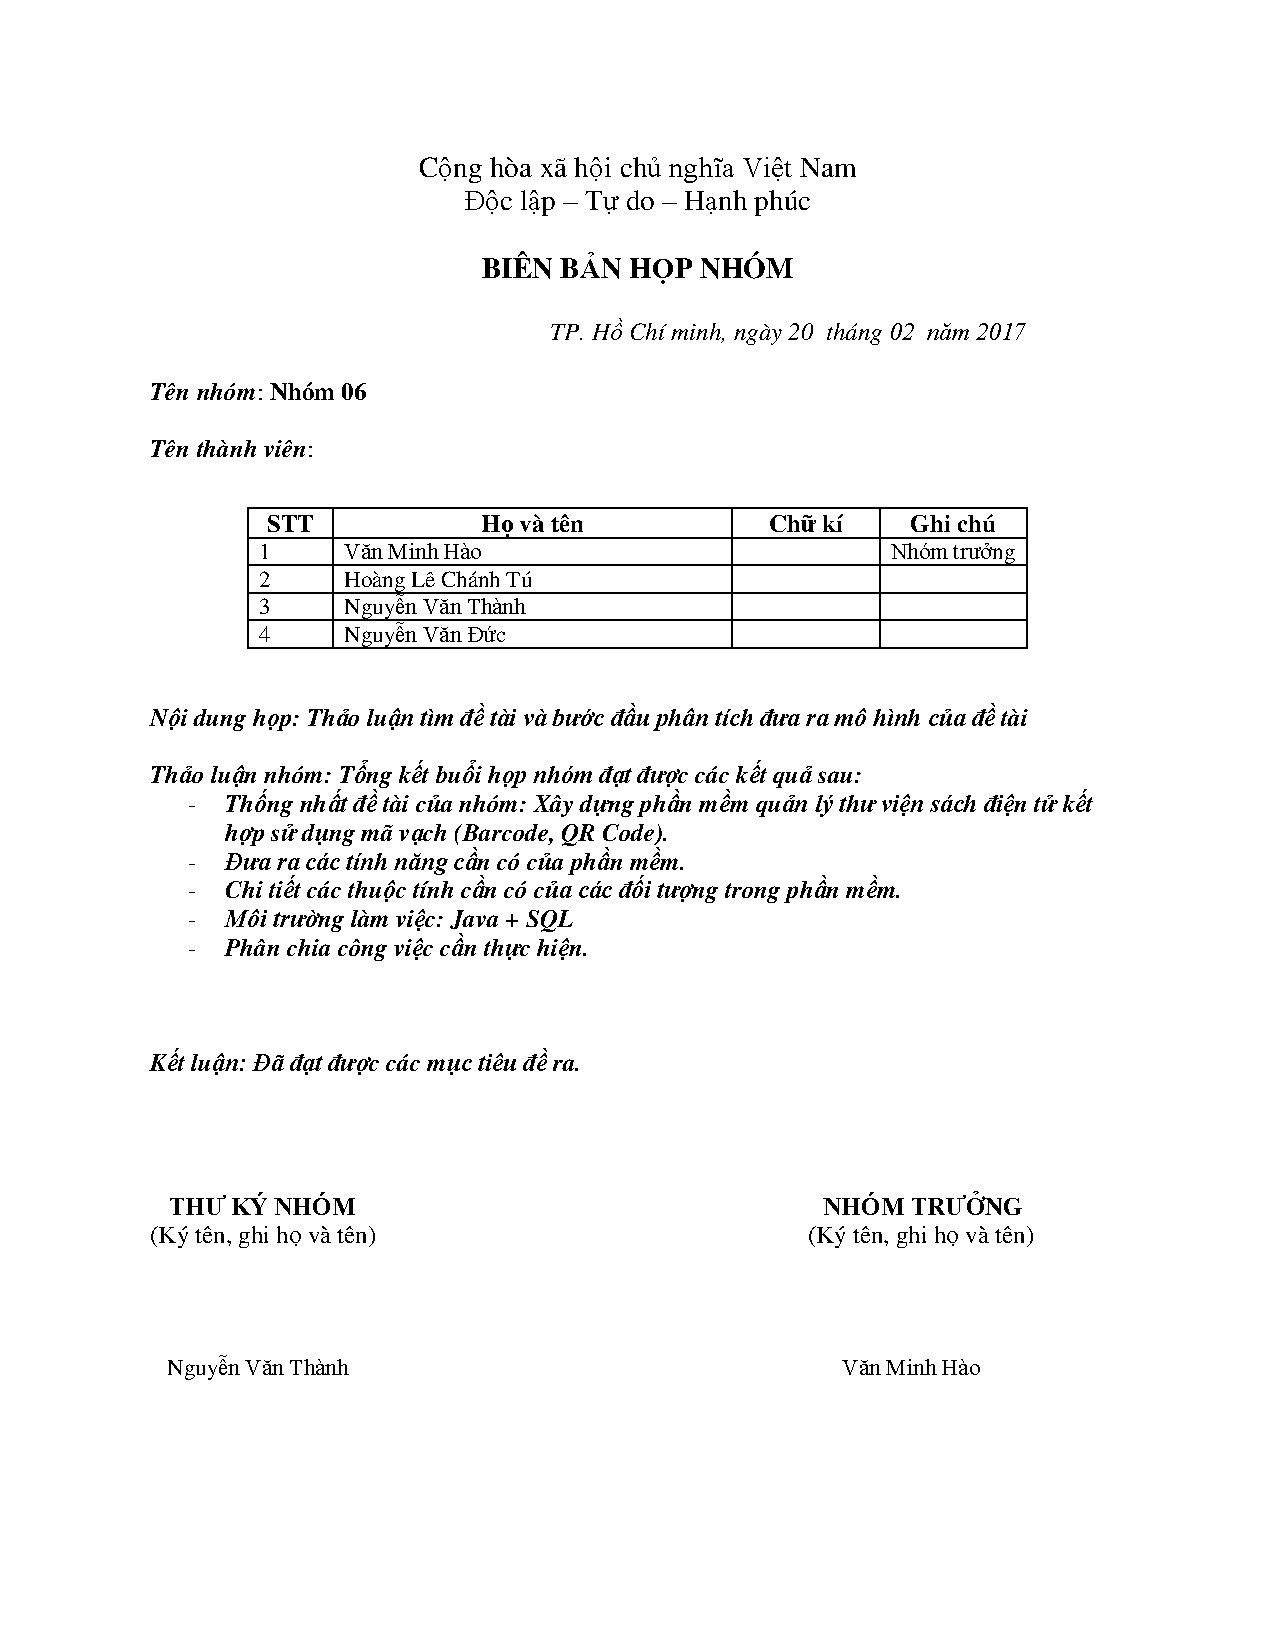
\includegraphics[scale=0.8]{images/hopnhomlan1.pdf}
			\end{figure}
			\addcontentsline{lof}{section}{Lần họp thứ hai}
			\begin{figure}[H]
			\centering
			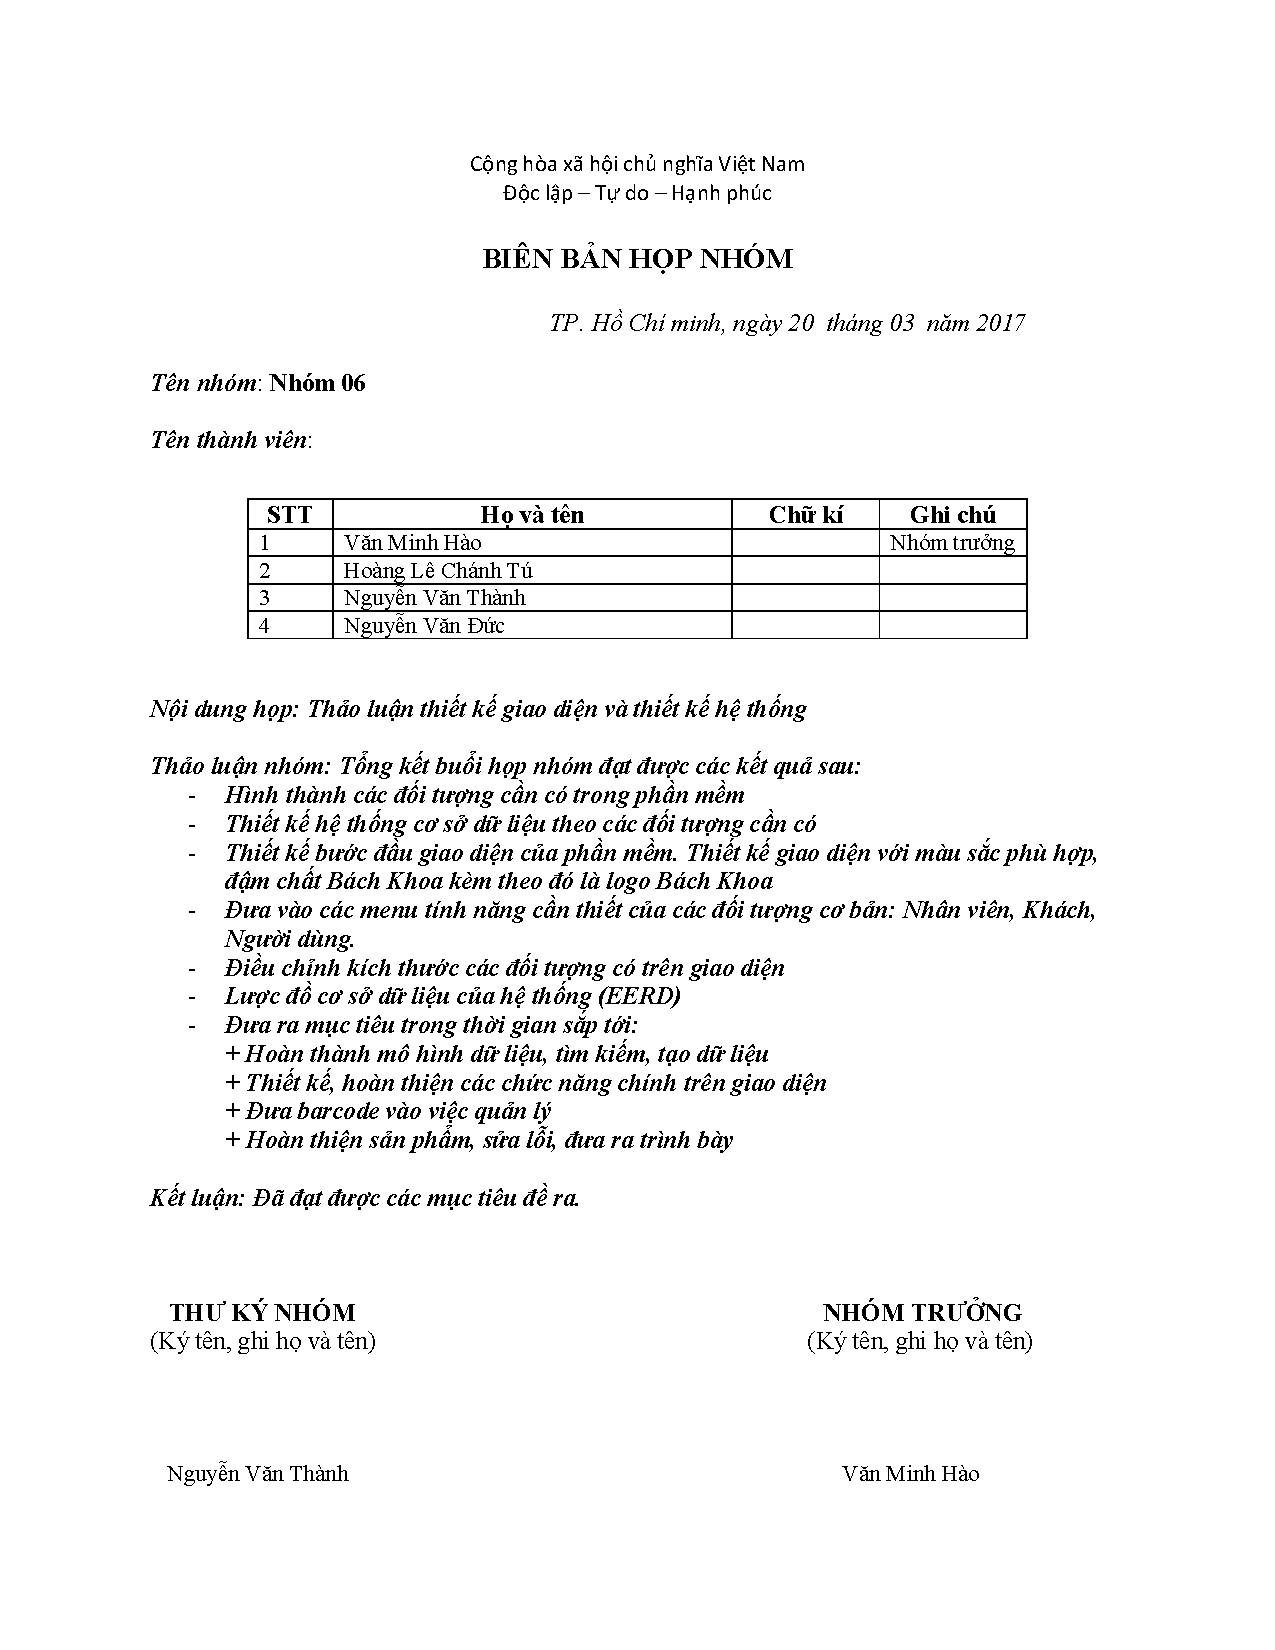
\includegraphics[scale=0.8]{images/hopnhomlan2.pdf}
			\end{figure}
			\addcontentsline{lof}{section}{Lần họp thứ ba}
			\begin{figure}[H]
			\centering
			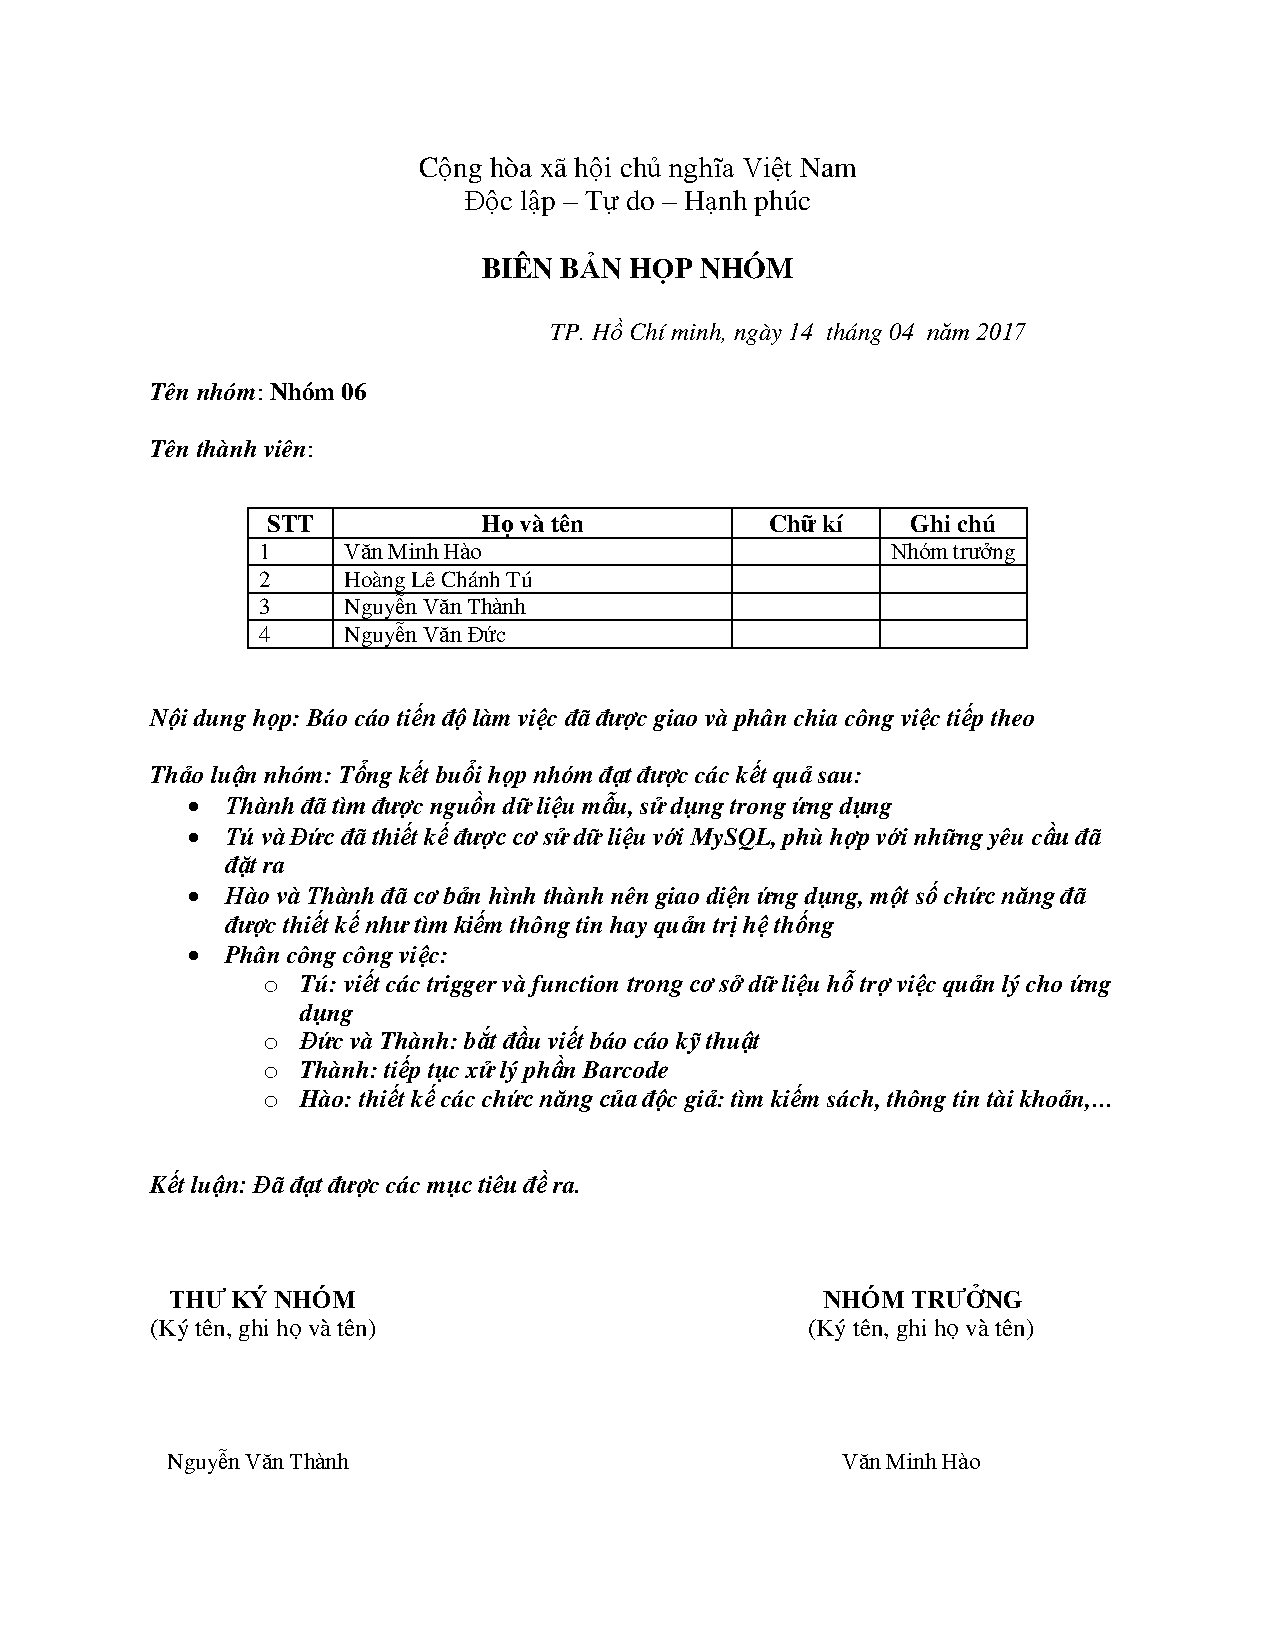
\includegraphics[scale=0.8]{images/hopnhomlan3.pdf}
			\end{figure}
			\addcontentsline{lof}{section}{Lần họp thứ tư}
			\begin{figure}[H]
			\centering
			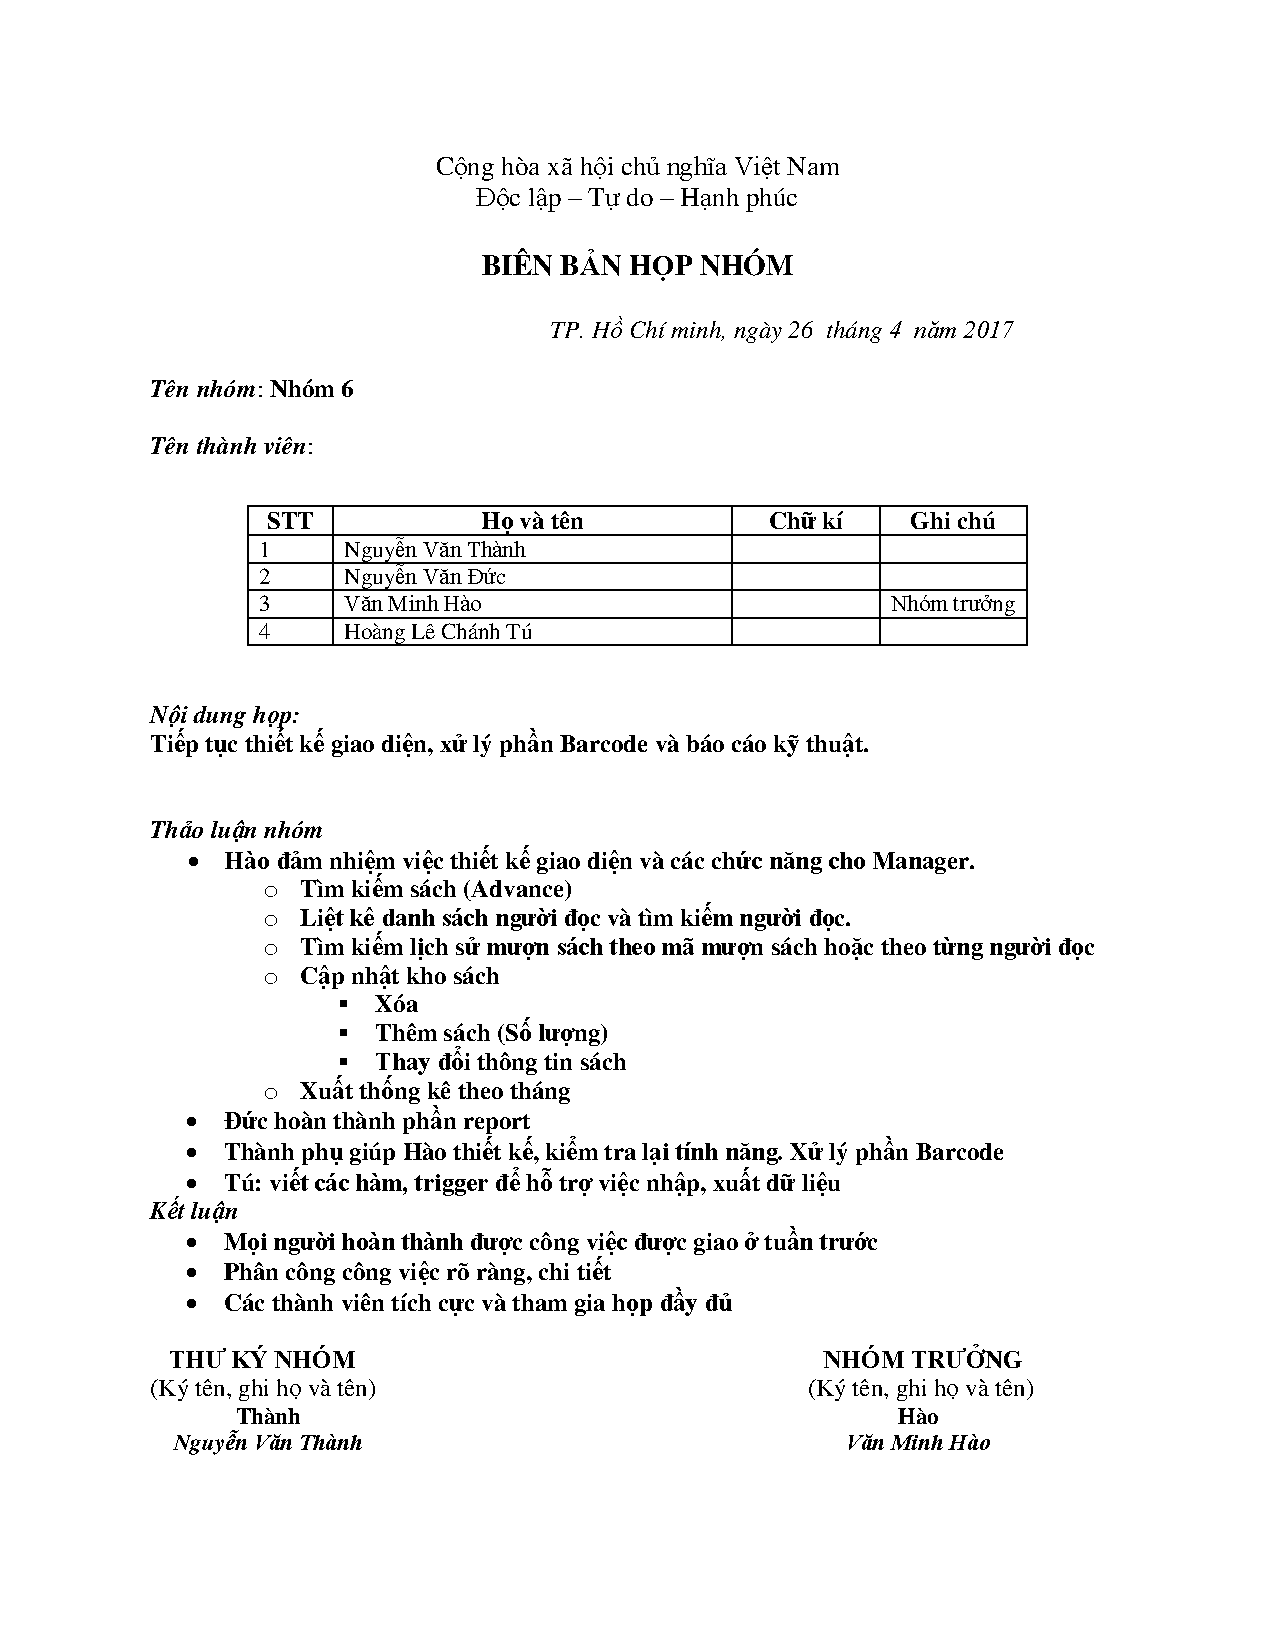
\includegraphics[scale=0.8]{images/hopnhomlan6.pdf}
			\end{figure}
			\addcontentsline{lof}{section}{Lần họp Cuối cùng}
			\begin{figure}[H]
			\centering
			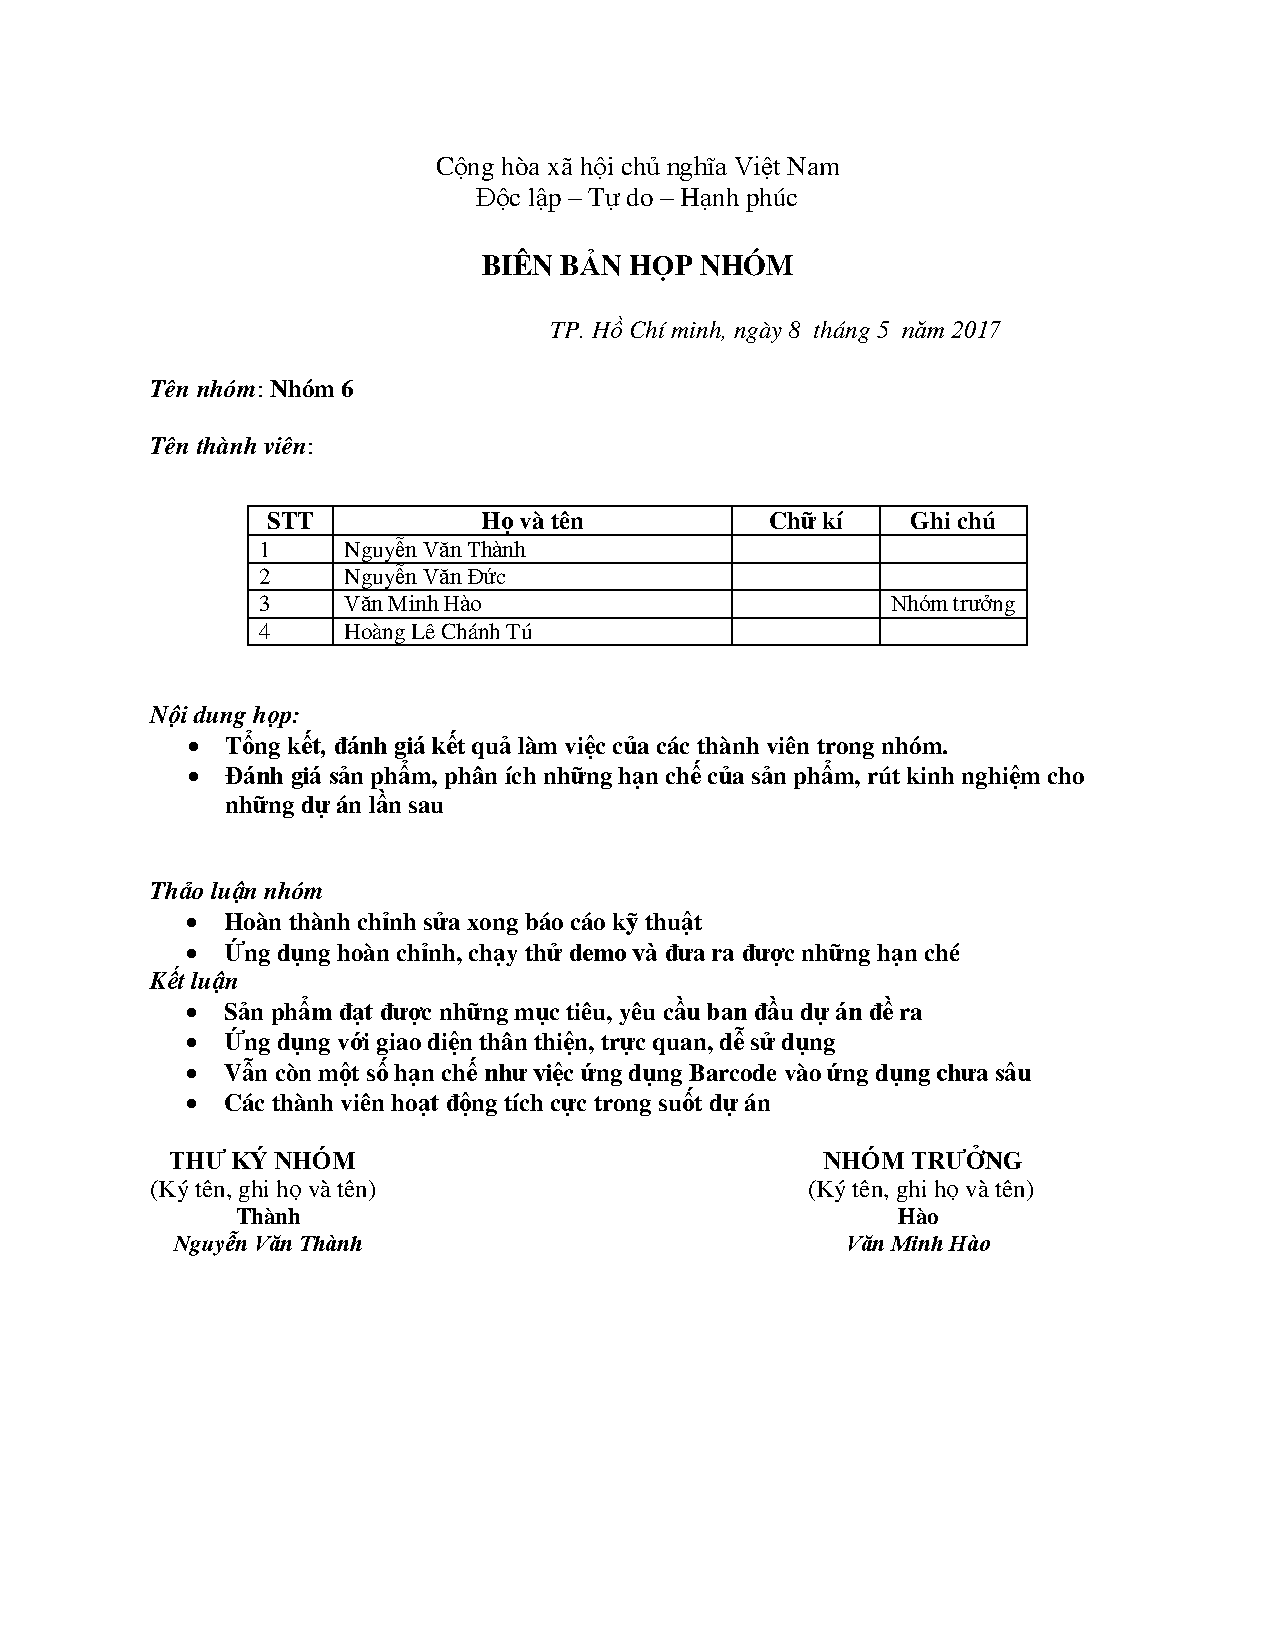
\includegraphics[scale=0.8]{images/hopnhomlan7.pdf}
			\end{figure}
		
		
\end{document}
